% Options for packages loaded elsewhere
\PassOptionsToPackage{unicode}{hyperref}
\PassOptionsToPackage{hyphens}{url}
\PassOptionsToPackage{dvipsnames,svgnames,x11names}{xcolor}
%
\documentclass[
  letterpaper,
  DIV=11,
  numbers=noendperiod]{scrreprt}

\usepackage{amsmath,amssymb}
\usepackage{iftex}
\ifPDFTeX
  \usepackage[T1]{fontenc}
  \usepackage[utf8]{inputenc}
  \usepackage{textcomp} % provide euro and other symbols
\else % if luatex or xetex
  \usepackage{unicode-math}
  \defaultfontfeatures{Scale=MatchLowercase}
  \defaultfontfeatures[\rmfamily]{Ligatures=TeX,Scale=1}
\fi
\usepackage{lmodern}
\ifPDFTeX\else  
    % xetex/luatex font selection
\fi
% Use upquote if available, for straight quotes in verbatim environments
\IfFileExists{upquote.sty}{\usepackage{upquote}}{}
\IfFileExists{microtype.sty}{% use microtype if available
  \usepackage[]{microtype}
  \UseMicrotypeSet[protrusion]{basicmath} % disable protrusion for tt fonts
}{}
\makeatletter
\@ifundefined{KOMAClassName}{% if non-KOMA class
  \IfFileExists{parskip.sty}{%
    \usepackage{parskip}
  }{% else
    \setlength{\parindent}{0pt}
    \setlength{\parskip}{6pt plus 2pt minus 1pt}}
}{% if KOMA class
  \KOMAoptions{parskip=half}}
\makeatother
\usepackage{xcolor}
\setlength{\emergencystretch}{3em} % prevent overfull lines
\setcounter{secnumdepth}{5}
% Make \paragraph and \subparagraph free-standing
\ifx\paragraph\undefined\else
  \let\oldparagraph\paragraph
  \renewcommand{\paragraph}[1]{\oldparagraph{#1}\mbox{}}
\fi
\ifx\subparagraph\undefined\else
  \let\oldsubparagraph\subparagraph
  \renewcommand{\subparagraph}[1]{\oldsubparagraph{#1}\mbox{}}
\fi

\usepackage{color}
\usepackage{fancyvrb}
\newcommand{\VerbBar}{|}
\newcommand{\VERB}{\Verb[commandchars=\\\{\}]}
\DefineVerbatimEnvironment{Highlighting}{Verbatim}{commandchars=\\\{\}}
% Add ',fontsize=\small' for more characters per line
\usepackage{framed}
\definecolor{shadecolor}{RGB}{241,243,245}
\newenvironment{Shaded}{\begin{snugshade}}{\end{snugshade}}
\newcommand{\AlertTok}[1]{\textcolor[rgb]{0.68,0.00,0.00}{#1}}
\newcommand{\AnnotationTok}[1]{\textcolor[rgb]{0.37,0.37,0.37}{#1}}
\newcommand{\AttributeTok}[1]{\textcolor[rgb]{0.40,0.45,0.13}{#1}}
\newcommand{\BaseNTok}[1]{\textcolor[rgb]{0.68,0.00,0.00}{#1}}
\newcommand{\BuiltInTok}[1]{\textcolor[rgb]{0.00,0.23,0.31}{#1}}
\newcommand{\CharTok}[1]{\textcolor[rgb]{0.13,0.47,0.30}{#1}}
\newcommand{\CommentTok}[1]{\textcolor[rgb]{0.37,0.37,0.37}{#1}}
\newcommand{\CommentVarTok}[1]{\textcolor[rgb]{0.37,0.37,0.37}{\textit{#1}}}
\newcommand{\ConstantTok}[1]{\textcolor[rgb]{0.56,0.35,0.01}{#1}}
\newcommand{\ControlFlowTok}[1]{\textcolor[rgb]{0.00,0.23,0.31}{#1}}
\newcommand{\DataTypeTok}[1]{\textcolor[rgb]{0.68,0.00,0.00}{#1}}
\newcommand{\DecValTok}[1]{\textcolor[rgb]{0.68,0.00,0.00}{#1}}
\newcommand{\DocumentationTok}[1]{\textcolor[rgb]{0.37,0.37,0.37}{\textit{#1}}}
\newcommand{\ErrorTok}[1]{\textcolor[rgb]{0.68,0.00,0.00}{#1}}
\newcommand{\ExtensionTok}[1]{\textcolor[rgb]{0.00,0.23,0.31}{#1}}
\newcommand{\FloatTok}[1]{\textcolor[rgb]{0.68,0.00,0.00}{#1}}
\newcommand{\FunctionTok}[1]{\textcolor[rgb]{0.28,0.35,0.67}{#1}}
\newcommand{\ImportTok}[1]{\textcolor[rgb]{0.00,0.46,0.62}{#1}}
\newcommand{\InformationTok}[1]{\textcolor[rgb]{0.37,0.37,0.37}{#1}}
\newcommand{\KeywordTok}[1]{\textcolor[rgb]{0.00,0.23,0.31}{#1}}
\newcommand{\NormalTok}[1]{\textcolor[rgb]{0.00,0.23,0.31}{#1}}
\newcommand{\OperatorTok}[1]{\textcolor[rgb]{0.37,0.37,0.37}{#1}}
\newcommand{\OtherTok}[1]{\textcolor[rgb]{0.00,0.23,0.31}{#1}}
\newcommand{\PreprocessorTok}[1]{\textcolor[rgb]{0.68,0.00,0.00}{#1}}
\newcommand{\RegionMarkerTok}[1]{\textcolor[rgb]{0.00,0.23,0.31}{#1}}
\newcommand{\SpecialCharTok}[1]{\textcolor[rgb]{0.37,0.37,0.37}{#1}}
\newcommand{\SpecialStringTok}[1]{\textcolor[rgb]{0.13,0.47,0.30}{#1}}
\newcommand{\StringTok}[1]{\textcolor[rgb]{0.13,0.47,0.30}{#1}}
\newcommand{\VariableTok}[1]{\textcolor[rgb]{0.07,0.07,0.07}{#1}}
\newcommand{\VerbatimStringTok}[1]{\textcolor[rgb]{0.13,0.47,0.30}{#1}}
\newcommand{\WarningTok}[1]{\textcolor[rgb]{0.37,0.37,0.37}{\textit{#1}}}

\providecommand{\tightlist}{%
  \setlength{\itemsep}{0pt}\setlength{\parskip}{0pt}}\usepackage{longtable,booktabs,array}
\usepackage{calc} % for calculating minipage widths
% Correct order of tables after \paragraph or \subparagraph
\usepackage{etoolbox}
\makeatletter
\patchcmd\longtable{\par}{\if@noskipsec\mbox{}\fi\par}{}{}
\makeatother
% Allow footnotes in longtable head/foot
\IfFileExists{footnotehyper.sty}{\usepackage{footnotehyper}}{\usepackage{footnote}}
\makesavenoteenv{longtable}
\usepackage{graphicx}
\makeatletter
\def\maxwidth{\ifdim\Gin@nat@width>\linewidth\linewidth\else\Gin@nat@width\fi}
\def\maxheight{\ifdim\Gin@nat@height>\textheight\textheight\else\Gin@nat@height\fi}
\makeatother
% Scale images if necessary, so that they will not overflow the page
% margins by default, and it is still possible to overwrite the defaults
% using explicit options in \includegraphics[width, height, ...]{}
\setkeys{Gin}{width=\maxwidth,height=\maxheight,keepaspectratio}
% Set default figure placement to htbp
\makeatletter
\def\fps@figure{htbp}
\makeatother
% definitions for citeproc citations
\NewDocumentCommand\citeproctext{}{}
\NewDocumentCommand\citeproc{mm}{%
  \begingroup\def\citeproctext{#2}\cite{#1}\endgroup}
\makeatletter
 % allow citations to break across lines
 \let\@cite@ofmt\@firstofone
 % avoid brackets around text for \cite:
 \def\@biblabel#1{}
 \def\@cite#1#2{{#1\if@tempswa , #2\fi}}
\makeatother
\newlength{\cslhangindent}
\setlength{\cslhangindent}{1.5em}
\newlength{\csllabelwidth}
\setlength{\csllabelwidth}{3em}
\newenvironment{CSLReferences}[2] % #1 hanging-indent, #2 entry-spacing
 {\begin{list}{}{%
  \setlength{\itemindent}{0pt}
  \setlength{\leftmargin}{0pt}
  \setlength{\parsep}{0pt}
  % turn on hanging indent if param 1 is 1
  \ifodd #1
   \setlength{\leftmargin}{\cslhangindent}
   \setlength{\itemindent}{-1\cslhangindent}
  \fi
  % set entry spacing
  \setlength{\itemsep}{#2\baselineskip}}}
 {\end{list}}
\usepackage{calc}
\newcommand{\CSLBlock}[1]{\hfill\break\parbox[t]{\linewidth}{\strut\ignorespaces#1\strut}}
\newcommand{\CSLLeftMargin}[1]{\parbox[t]{\csllabelwidth}{\strut#1\strut}}
\newcommand{\CSLRightInline}[1]{\parbox[t]{\linewidth - \csllabelwidth}{\strut#1\strut}}
\newcommand{\CSLIndent}[1]{\hspace{\cslhangindent}#1}

\KOMAoption{captions}{tableheading}
\makeatletter
\@ifpackageloaded{bookmark}{}{\usepackage{bookmark}}
\makeatother
\makeatletter
\@ifpackageloaded{caption}{}{\usepackage{caption}}
\AtBeginDocument{%
\ifdefined\contentsname
  \renewcommand*\contentsname{Table of contents}
\else
  \newcommand\contentsname{Table of contents}
\fi
\ifdefined\listfigurename
  \renewcommand*\listfigurename{List of Figures}
\else
  \newcommand\listfigurename{List of Figures}
\fi
\ifdefined\listtablename
  \renewcommand*\listtablename{List of Tables}
\else
  \newcommand\listtablename{List of Tables}
\fi
\ifdefined\figurename
  \renewcommand*\figurename{Figure}
\else
  \newcommand\figurename{Figure}
\fi
\ifdefined\tablename
  \renewcommand*\tablename{Table}
\else
  \newcommand\tablename{Table}
\fi
}
\@ifpackageloaded{float}{}{\usepackage{float}}
\floatstyle{ruled}
\@ifundefined{c@chapter}{\newfloat{codelisting}{h}{lop}}{\newfloat{codelisting}{h}{lop}[chapter]}
\floatname{codelisting}{Listing}
\newcommand*\listoflistings{\listof{codelisting}{List of Listings}}
\makeatother
\makeatletter
\makeatother
\makeatletter
\@ifpackageloaded{caption}{}{\usepackage{caption}}
\@ifpackageloaded{subcaption}{}{\usepackage{subcaption}}
\makeatother
\ifLuaTeX
  \usepackage{selnolig}  % disable illegal ligatures
\fi
\usepackage{bookmark}

\IfFileExists{xurl.sty}{\usepackage{xurl}}{} % add URL line breaks if available
\urlstyle{same} % disable monospaced font for URLs
\hypersetup{
  pdftitle={MATH337: Changepoint Detection},
  pdfauthor={Gaetano Romano},
  colorlinks=true,
  linkcolor={blue},
  filecolor={Maroon},
  citecolor={Blue},
  urlcolor={Blue},
  pdfcreator={LaTeX via pandoc}}

\title{MATH337: Changepoint Detection}
\author{Gaetano Romano}
\date{2024-11-01}

\begin{document}
\maketitle

\renewcommand*\contentsname{Table of contents}
{
\hypersetup{linkcolor=}
\setcounter{tocdepth}{2}
\tableofcontents
}
\bookmarksetup{startatroot}

\chapter*{Preface}\label{preface}
\addcontentsline{toc}{chapter}{Preface}

\markboth{Preface}{Preface}

These are the notes for \textbf{MATH337 Changepoint Detection}. They
were written by \href{https://www.lancaster.ac.uk/~romano/}{Gaetano
Romano}.

The module will introduce you to changepoint detection, detailing some
algorithms, developing the basics theoretical foundations, and
practicing few real-world scenarios.

Across five weeks we will cover the following topics:

\begin{enumerate}
\def\labelenumi{\arabic{enumi}.}
\item
  An introduction to changepoint detection and the CUSUM statistics
\item
  Controlling the CUSUM and some additional models
\item
  Dealing with multiple changes
\item
  PELT, WBS and Penalty selection
\item
  Working with Real World data.
\end{enumerate}

We will be using R as the programming language for this module. If
you're unfamiliar with it, make sure you cover the first three weeks of
\href{https://lumath245.github.io/_book/index.html}{MATH245}.

Every week, you are expected to follow two lectures, one workshop, and
one computer aided lab. Over the lecture, we will cover the basics
concepts of changepoint detection.

At the end of each chapter, you will find exercises that will be carried
in the workshop and the lab. During the workshop, you will be dealing
with computations and details about the methodologies introduced at your
own pace, and, finally, during the workshops, you'll give a go at
programming the various algorithms and running real-world examples.

\textbf{You will find the solutions to the exercises on the Moodle page,
released weekly}. If you cannot access the Moodle page, and you still
would like to have these solutions, please get in touch with me.

\section*{Source files, and
attributions}\label{source-files-and-attributions}
\addcontentsline{toc}{section}{Source files, and attributions}

\markright{Source files, and attributions}

The notes are released as open-source on GitHub under the
\href{https://github.com/gtromano/MATH337_changepoint_detection?tab=License-1-ov-file}{CC
BY-NC 4.0 License}. You can access the repository at the following link:
\url{https://github.com/gtromano/MATH337_changepoint_detection}.

The materials in this course are based on and share elements with the
following resources:

\begin{itemize}
\tightlist
\item
  Fearnhead, P., \& Fryzlewicz, P. (2022). Detecting a single
  change-point. \emph{arXiv preprint arXiv:2210.07066}.
\item
  \href{https://github.com/rkillick/intro-changepoint-course}{Rebecca
  Killick's Introduction to Changepoint Detection} - a half-day
  introductory course on changepoint detection.
\item
  \href{https://github.com/rkillick/further-changepoints-course}{Rebecca
  Killick's Further Changepoint Topics} - an extended course on
  changepoint detection.
\item
  \href{https://github.com/tdhock/2023-08-unsupervised-learning}{Toby
  Hocking's Course on Unsupervised Learning}, which includes changepoint
  detection.
\end{itemize}

I would like to express my gratitude to the authors of these resources.
In addition, materials were sourced from various academic papers, which
are referenced throughout the body of these notes.

\bookmarksetup{startatroot}

\chapter{An Introduction to Changepoint
Detection}\label{an-introduction-to-changepoint-detection}

\section{Piecewise Stationary Time
Series}\label{piecewise-stationary-time-series}

In this module, we will be dealing with \textbf{time series}. A time
series is a sequence of observations recorded over time (or space),
where the order of the data points is crucial.

\subsection{What is a time series?}\label{what-is-a-time-series}

In previous modules, such as Likelihood Inference, we typically dealt
with data that was not ordered in a particular way. For example, we
might have worked with a sample of independent Gaussian observations,
where each observation is drawn randomly from the same distribution.
This sample might look like the following:

\[
  y_i \sim \mathcal{N}(0,1), \ i = 1, \dots, 100
\]

Here, \(y_i\) represents the \(i\)-th observation, and the assumption is
that all observations are independent and identically distributed
(i.i.d.) with a mean of 0 and variance of 1.

\includegraphics{1_intro_cusum_files/figure-pdf/unnamed-chunk-2-1.pdf}

In this case, the observations do not have any particular order, and our
primary interest may be in estimating parameters such as the mean,
variance, or mode of the distribution. This is typical for traditional
inference, where the order of observations is not of concern.

However, a \textbf{time series} involves a specific order to the
data---usually indexed by time, although it could also be by space or
another sequential dimension. For example, we could assume that the
Gaussian sample above is a sequential process, ordered by the time we
drew an observation. Each observation corresponds to a specific time
point \(t\):

\includegraphics{1_intro_cusum_files/figure-pdf/unnamed-chunk-3-1.pdf}

\textbf{Formal Notation.} In time series analysis, we typically denote a
time series by using an index \(t\) to represent time or order. The time
series vector is written as:

\[
  y_{1:n} = (y_1, y_2, \dots, y_n)
\]

Here, \(n\) is the total length of the sequence, and \(y_t\) represents
the observed value at time \(t\), for \(t = 1, 2, \dots, n\). In our
previous example, for instance, \(n = 100\).

Often, we are also interested in subsets of a time series (inclusive),
especially when investigating specific ``windows'' or ``chunks'' of the
data. We will denote as a subset of the time series, from time \(l\) to
time \(u\), the following:

\[
  y_{l:u} = (y_l, y_{l+1}, \dots, y_u)
\]

Understanding and working with subsets of time series data is important
for many applications, such as when detecting changes in the behavior or
properties of the time series over specific intervals.

\subsection{Stationary, non-stationary, and piecewise stationary time
series}\label{stationary-non-stationary-and-piecewise-stationary-time-series}

Time series can be classified into different categories based on their
statistical properties over time. The three main types are
\textbf{stationary}, \textbf{non-stationary}, and \textbf{piecewise
stationary} time series. For example:

\includegraphics{1_intro_cusum_files/figure-pdf/unnamed-chunk-4-1.pdf}

\begin{enumerate}
\def\labelenumi{\arabic{enumi}.}
\tightlist
\item
  \textbf{Stationary Time Series}: A time series is said to be
  \emph{stationary} if its statistical properties---such as the mean,
  variance, and autocovariance---are constant over time. This implies
  that the behavior of the series doesn't change as time progresses.
\end{enumerate}

Mathematically, for a stationary time series \(y_t\), the expected value
and variance are constant over time: \[
    \mathbb{E}(y_t) = \mu \quad \text{and} \quad \text{Var}(y_t) = \sigma^2 \quad \forall \in \{1, ..., n\}
\] In this example, the stationary time series was generated by sampling
random normal variables
\(y_t = \epsilon_t, \ \epsilon_t \sim \mathcal{N}(0, 1)\). We can see,
very simply how, in this case: \[
    \mathbb{E}(y_t) = \mathbb{E}(\epsilon_t) = 0, \forall t \in \{1, ..., 100\}
\]

\begin{enumerate}
\def\labelenumi{\arabic{enumi}.}
\setcounter{enumi}{1}
\tightlist
\item
  \textbf{Non-Stationary Time Series}: A time series is
  \emph{non-stationary} if its statistical properties change over time.
  Often, non-stationary series exhibit trends or varying variances. For
  example, a series with a trend (increasing or decreasing) is
  non-stationary because the mean is not constant.
\end{enumerate}

A common form of non-stationarity is a linear trend, where the series
grows over time. In our example, the non-stationary series is generated
as: \[
    y_t = \epsilon_t + 0.1 \cdot t , \ \epsilon_t \sim \mathcal{N}(0, 1)
\] This creates a time series with a linear upward trend. In fact,
similarly to what done before: \[
    \mathbb{E}(y_t) = \mathbb{E}(\epsilon_t) + \mathbb{E}(0.1 \cdot t) = 0.1 \cdot t. 
\] Therefore: \[
  \forall t_1, t_2 \in \{1, ..., 100\}, t_1 \neq t_2 \rightarrow \mathbb{E}(y_{t_1}) \neq \mathbb{E}(y_{t_2})
\]

\begin{enumerate}
\def\labelenumi{\arabic{enumi}.}
\setcounter{enumi}{2}
\tightlist
\item
  \textbf{Piecewise Stationary Time Series}: A \emph{piecewise
  stationary} time series is stationary within certain segments but has
  changes in its statistical properties at certain points, known as
  \emph{changepoints}. After each changepoint, the series may have a
  different mean, variance, or both.
\end{enumerate}

In our example, the time series was stationary for the first half of the
observations, but after \(t = 50\), a sudden shift occurs.
Mathematically: \[
y_t = \begin{cases} 
    \epsilon_t & \text{for } t \leq 50 \\
    \epsilon_t + 5 & \text{for } t > 50
    \end{cases}, \quad \epsilon_t \sim \mathcal{N}(0, 1)
\] This abrupt change at \(t = 50\) introduces a piecewise structure to
the data.

\section{Introduction to
changepoints}\label{introduction-to-changepoints}

Changepoints are sudden, and often unexpected, shifts in the behavior of
a process. They are also known as breakpoints, structural breaks, or
regime switches. The detection of changepoints is crucial in
understanding and responding to changes in various types of time series
data.

The primary objectives in detecting changepoints include:

\begin{itemize}
\tightlist
\item
  \textbf{Has a change occurred?}: Identifying if there is a shift in
  the data.
\item
  \textbf{If yes, where is the change?}: Locating the precise point
  where the change happened.
\item
  \textbf{What is the difference between the pre and post-change data?}
  This may reveal the type of change, and it could indicate differences
  in parameter values before and after the change.
\item
  \textbf{How certain are we of the changepoint location?}: Assessing
  the confidence in the detected changepoint.
\item
  \textbf{How many changes have occurred?}: Identifying multiple
  changepoints and analyzing each one for similar characteristics.
\end{itemize}

Changepoints can be found in a wide range of time series, not limited to
physical, biological, industrial, or financial processes, and which
objectives to follow depends on the type of the analysis we are
carrying.

In changepoint detection, there are two main approaches: \textbf{online}
and \textbf{offline} analysis. In applications that require
\textbf{online analysis}, the data is processed as it arrives, or in
small batches. The primary goal of online changepoint detection is to
identify changes as quickly as possible, making it crucial in contexts
such as process control or intrusion detection, where immediate action
is necessary.

On the other hand, \textbf{offline analysis} processes all the data at
once, typically after it has been fully collected. The aim here is to
provide an accurate detection of changepoints, rather than a rapid one.
This approach is common in fields like genome analysis or audiology,
where the focus is on understanding the structure of the data
post-collection.

For instance, to give few examples:

\begin{enumerate}
\def\labelenumi{\arabic{enumi}.}
\item
  \textbf{ECG}: Detecting changes or abnormalities in electrocardiogram
  (ECG) data can help in diagnosing heart conditions.

  \begin{figure}[H]

  {\centering 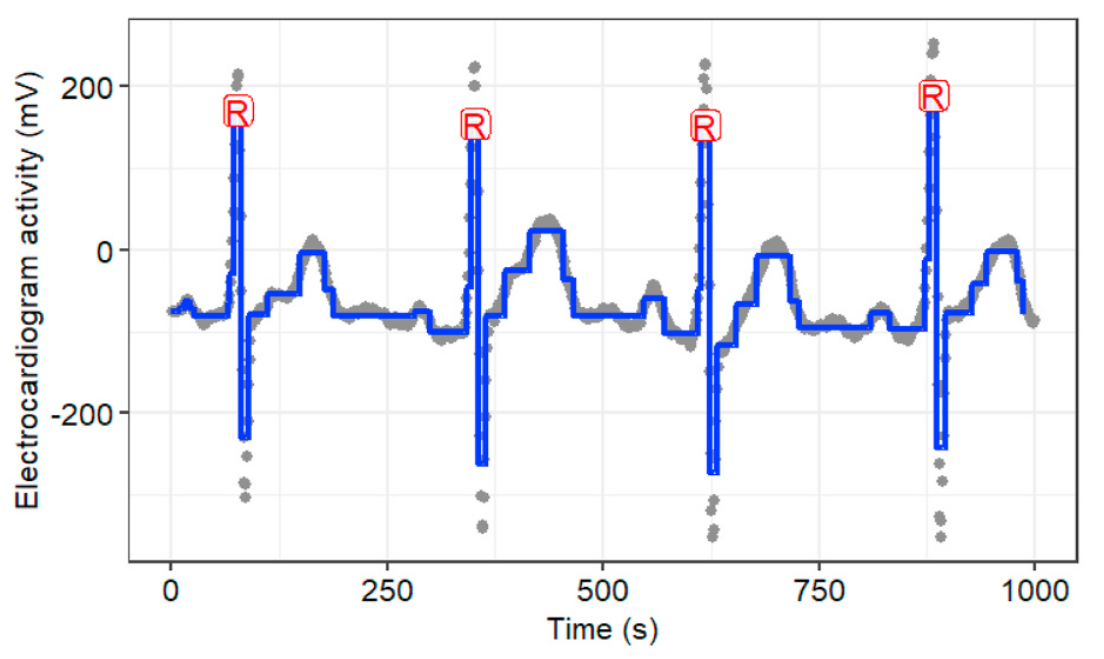
\includegraphics{source_imgs/intro-ecg.png}

  }

  \caption{Electrocardiograms (heart monitoring), Fotoohinasab et al,
  Asilomar conference 2020.}

  \end{figure}%
\item
  \textbf{Cancer Diagnosis}: Identifying breakpoints in DNA copy number
  data is important for diagnosing some types of cancer, such as
  neuroblastoma. This is a typical example of an offline analysis.

  \begin{figure}[H]

  {\centering 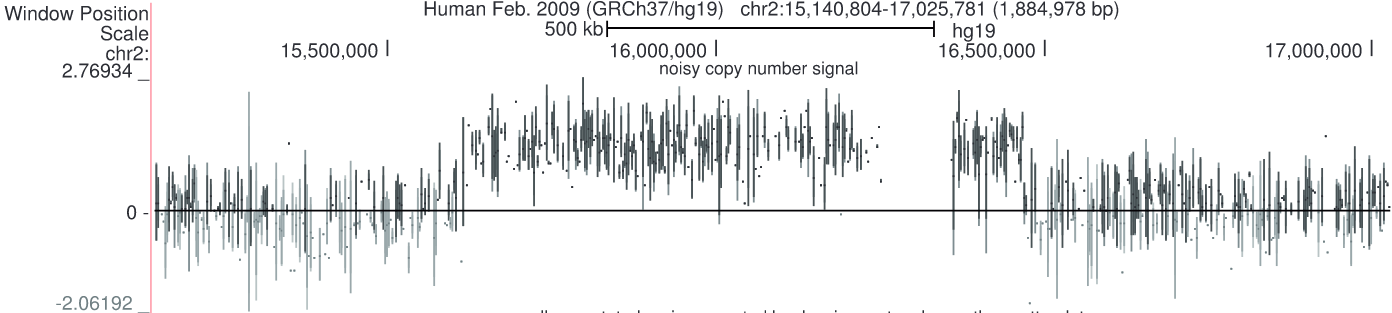
\includegraphics{source_imgs/intro-breakpoints.png}

  }

  \caption{DNA copy number data, breakpoints associated with aggressive
  cancer, Hocking et al, Bioinformatics 2014.}

  \end{figure}%
\item
  \textbf{Engineering Monitoring}: Detecting changes in CPU monitoring
  data in servers can help in identifying potential issues or failures:
  this is often analysed in real-time on with online methods, with the
  aim of detecting an issue as quickly as possible.

  \begin{figure}[H]

  {\centering 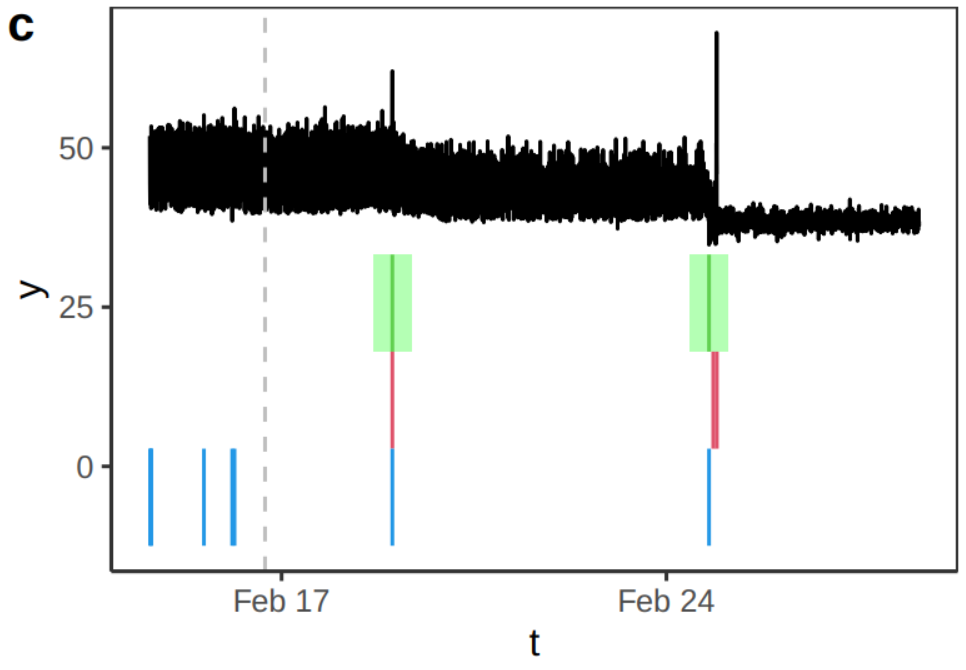
\includegraphics{source_imgs/CPU-monitoring.png}

  }

  \caption{Temperature data from a CPU of an AWS server. Source Romano
  et al., (2023)}

  \end{figure}%
\end{enumerate}

In this module, we will focus exclusively on \textbf{offline}
changepoint detection, where we assume that all the data is available
for analysis from the start.

\subsection{Types of Changes in Time
Series}\label{types-of-changes-in-time-series}

As you might have noticed from the examples above, there's not a strict
way on which a time-series might change. Depending on the model, we
could seek for different types of changes in the structure of a time
series. Some of the most common types of changes include shifts in mean,
variance, and trends in regression. For example, the CPU example above
exihibited, in addition to some extreme observations, both changes in
mean and variance.

\begin{itemize}
\tightlist
\item
  A \textbf{change in mean} occurs when the average level of an
  otherwise stationary time series shifts from one point to another.
  This type of change is often encountered in real-world data when there
  is a sudden shift in the process generating the data, such as a change
  in policy, market conditions, or external factors affecting the
  system.
\end{itemize}

\includegraphics{1_intro_cusum_files/figure-pdf/unnamed-chunk-5-1.pdf}

In the plot above, the red lines indicate the true mean values of the
different segments.

\begin{itemize}
\tightlist
\item
  A \textbf{change in variance} refers to a shift in the variability of
  the time series data, even when the mean remains constant. This type
  of change is important in scenarios where the stability of a process
  fluctuates over time. For example, in financial markets, periods of
  high volatility (high variance) may be followed by periods of relative
  calm (low variance).
\end{itemize}

\includegraphics{1_intro_cusum_files/figure-pdf/unnamed-chunk-6-1.pdf}

\subsubsection{3. Change in Regression
(Slope)}\label{change-in-regression-slope}

A \textbf{change in regression} or slope occurs when the underlying
relationship between time and the values of the time series changes.
This could reflect a shift in the growth or decline rate of a process.
For example, a company's revenue might grow steadily over a period, then
plateau, and later exhibit a quadratic or nonlinear growth trend.

\includegraphics{1_intro_cusum_files/figure-pdf/unnamed-chunk-7-1.pdf}

\subsection{The biggest data challenge in changepoint
detection}\label{the-biggest-data-challenge-in-changepoint-detection}

One of the most widely debated and difficult data challenges in
changepoint detection may not be in the field of finance, genetics, or
climate science---but rather in television history. Specifically, the
question that has plagued critics and fans alike for years is:
\textbf{At which episode did ``The Simpsons'' start to decline?}

It's almost common knowledge that ``The Simpsons,'' the longest-running
and most beloved animated sitcom, experienced a significant drop in
quality over time. But pinpointing exactly \emph{when} this drop
occurred is the real challenge. Fortunately, there's a branch of
statistics that was practically built to answer questions like these!

I have downloaded a dataset (Bown 2023) containing ratings for every
episode of ``The Simpsons'' up to season 34. We will analyze this data
to determine if and when a significant shift occurred in the ratings,
which might reflect the decline in quality that so many have observed.

\includegraphics{1_intro_cusum_files/figure-pdf/unnamed-chunk-8-1.pdf}

In this plot, each episode of ``The Simpsons'' is represented by its
TMBD rating, and episodes are colored by season. By visually inspecting
the graph, we may already start to see some potential points where the
ratings decline. However, the goal of our changepoint analysis is to
move beyond visual inspection and rigorously detect the exact moment
where a significant shift in the data occurs.

Jokes apart, this is a challenging time series! First of all, there's
not a clear single change, but rather an increase, followed by a
decline. After which, the sequence seems rather stationary. For this
reason, throughout the module, we will use this data as a running
example to develop our understanding of various methods, hopefully
trying to obtain a definitive answer towards the final chapters. But
let's proceed with order\ldots{}

\section{Detecting one change in
mean}\label{detecting-one-change-in-mean}

In this section, we will start by exploring the simplest case of a
changepoint detection problem: \textbf{detecting a change in the mean}
of a time series. We assume that the data is generated according to the
following model:

\[
y_t = \mu_t + \epsilon_t, \quad t = 1, \dots, n,
\]

where \(\epsilon_t \sim \mathcal{N}(0, \sigma^2)\) represents Gaussian
noise with mean 0 and known variance \(\sigma^2\), and
\(\mu_t \in \mathbb{R}\) is the signal at time \(t\). The vector of
noise terms \(\epsilon_{1:n}\) is often referred to as Gaussian noise,
and hence, this model is known as \emph{the signal plus noise model},
where the signal is given by \(\mu_{1:n}\) and the noise by
\(\epsilon_{1:n}\).

In \emph{the change-in-mean problem}, our goal is to determine whether
the signal remains constant throughout the entire sequence, or if there
exists a point \(\tau\)), where the mean shifts. In other words, we are
testing whether:

\[
\mu_1 = \mu_2 = \dots = \mu_n \quad \text{(no changepoint)},
\]

or if there exists a time \(\tau\) such that:

\[
\mu_1 = \mu_2 = \dots = \mu_\tau \neq \mu_{\tau+1} = \dots = \mu_n \quad \text{(changepoint at } \tau\text{)}.
\]

\textbf{Note.} The point \(\tau\) is our \emph{changepoint}, e.g.~the
first point after which our mean changes, however there's a lot of
inconsistencies on the literature: sometimes you will find that people
refer to \(\tau + 1\) as the changepoint, and \(\tau\) as the last
pre-change point (as a matter of fact, please let me know if you spot
this inconsistency anywhere in these notes!).

To address this problem, one of the most widely used methods is
\emph{the CUSUM (Cumulative Sum) statistic}. The basic idea behind the
CUSUM statistic is to systematically compare the distribution of the
data to the left and right of each possible changepoint \(\tau\). By
doing so, we can assess whether there is evidence of a significant
change in the mean at a given point.

\subsection{The CUSUM statistics}\label{the-cusum-statistics}

The CUSUM statistic works by comparing, for each potential data point,
the empirical mean (average) of the data to the left (before \(\tau\))
with the empirical mean of the data to the right (after \(\tau\)):

\[
C_{\tau} = \sqrt{\frac{\tau(n-\tau)}{n}} \left| \bar{y}_{1:\tau} - \bar{y}_{(\tau+1):n} \right|,
\]

Our \(\bar{y}_{1:\tau}\) and \(\bar{y}_{(\tau+1):n}\) are just the
empirical means of each segment, simply computed with:

\[
\bar{y}_{l:u} = \frac{1}{u - l + 1} \sum_{t = l}^{u} y_t.
\]

The term on the left of the difference, is there to re-scale it so that
our statistics is the absolute value of normal RV that has variance 1.
If there is no change, this difference is going to be distributed as a
standard normal, and this is going to be a key step in drawing the
distribution of the CUSUM statistic next week.

This approach is intuitive because if the mean \(\mu\) is the same
across the entire sequence, the values of the averages on both sides of
any point \(\tau\) should be similar. However, if there is a change in
the mean, the means will differ significantly, highlighting the
changepoint.

More formally, we would detect at change at \(\tau\) if:

\[
\frac{C_{\tau}^2 }{\sigma^2} > c,
\] where the \(c \in \mathbb{R}^+\) is a suitable chosen threshold value
(similar to a critical value in hypothesis testing!).

\subsection{\texorpdfstring{Searching for all
\(\tau\)s}{Searching for all \textbackslash taus}}\label{searching-for-all-taus}

In practice, however, we do not know the changepoint location in
advance. Our goal is to detect whether a changepoint exists and, if so,
estimate its location. To achieve this, we need to consider all possible
changepoint locations and choose the one that maximizes our test
statistic.

The natural extension of the likelihood-ratio test to this situation is
to use as a test statistic the maximum of \(C_\tau\) as we vary
\(\tau\):

\[
C_{max} = \max_{\tau \in \{1,\ldots,n-1\}} C_\tau^2 / \sigma^2
\]

And detect a changepoint if \(C_{max} > c\) for some suitably chosen
threshold \(c\). The choice of \(c\) will determine the significance
level of the test (we'll discuss this in more detail later).
Graphically, the test will look:

\includegraphics{1_intro_cusum_files/figure-pdf/unnamed-chunk-9-1.pdf}

If we detect a changepoint (i.e., if \(C_{max} > c\)), we can estimate
its location by:

\[
\hat{\tau} = \arg\max_{\tau \in \{1,\ldots,n-1\}}  C_\tau^2 / \sigma^2
\]

In other words, \(\hat{\tau}\) is the value of \(\tau\) that maximizes
the CUSUM statistic.

A simple estimate of the size of the change is then given by:

\[
\Delta\hat{\mu} = \bar{y}_{(\hat{\tau}+1):n} - \bar{y}_{1:\hat{\tau}}
\]

This estimate represents the difference between the mean of the data
after the estimated changepoint and the mean of the data before the
estimated changepoint.

\subsection{Example}\label{example}

Let us compute the cusum for the vector
\(y_{1:4} = (0.5, -0.1, 12.1, 12.4)\).

We know that \(n = 4\) (the total number of observations), therefore
possible changepoints include: \(\tau = 1, 2, 3\).

\textbf{Compute empirical means for each segment}

We first need to calculate the segment means, \(\bar{y}_{1:\tau}\) and
\(\bar{y}_{(\tau+1):n}\), for each \(\tau\).

\begin{itemize}
\item
  For \(\tau = 1\), the left segment is: \(y_{1:1} = \{0.5\}\), and
  \(\bar{y}_{1:1} = 0.5.\) The right segment:
  \(y_{2:4} = (-0.1, 12.1, 12.4)\) gives
  \(\bar{y}_{2:4} = \frac{-0.1 + 12.1 + 12.4}{3} = \frac{24.4}{3} = 8.13.\)
\item
  For \(\tau = 2\), we have, in a similar fashion,
  \(\bar{y}_{1:2} = \frac{0.5 - 0.1}{2} = 0.2.\),
  \(\bar{y}_{3:4} = \frac{12.1 + 12.4}{2} = 12.25\)
\item
  Lastly, for \(\tau = 3\), we have
  \(\bar{y}_{1:3} = \frac{0.5 - 0.1 + 12.1}{3} = \frac{12.5}{3} = 4.16\)
  and \(\bar{y}_{4:4} = 12.4\).
\end{itemize}

\textbf{Compute the CUSUM statistics}

Now that we have the empirical means for each segment, we have all the
ingredients for computing our CUSUM:

\[
C_{\tau} = \sqrt{\frac{\tau(n-\tau)}{n}} \left| \bar{y}_{1:\tau} - \bar{y}_{(\tau+1):n} \right|.
\]

\begin{itemize}
\item
  \textbf{For} \(\tau = 1\): \[
  C_1 = \sqrt{\frac{1(4-1)}{4}} \left| 0.5 - 8.13\overline{3} \right| = 0.866 \times 7.63\overline{3} = 6.61.
  \]
\item
  \textbf{For} \(\tau = 2\): \[
  C_2 = \sqrt{\frac{2(4-2)}{4}} \left| 0.2 - 12.25 \right| = 1 \times 12.05 = 12.05.
  \]
\item
  \textbf{For} \(\tau = 3\): \[
  C_3 = \sqrt{\frac{3(4-3)}{4}} \left| 4.16\overline{6} - 12.4 \right| = 0.866 \times 8.23\overline{3} = 7.13.
  \]
\end{itemize}

Thus, the maximum of the CUSUM statistic occurs at \(\tau = 2\), with
\(C_{max} = 12.05\). To detect a changepoint, we would compare
\(C_{max}\) to a threshold value \(c\). If \(C_{max} > c\), we conclude
that there is a changepoint at \(\hat{\tau} = 2\).

\subsection{Algorithmic Formulation of the CUSUM
Statistic}\label{algorithmic-formulation-of-the-cusum-statistic}

This process seems rather long, as for every step, we need to precompute
the means\ldots{} A naive implementation of the cusum, in fact, takes
\(\mathcal{O}(n^2)\) computations.

However, there's an algorithmic trick\ldots{} By sequentially computing
partial sums, e.g.~\(S_n = \sum_{i=1}^n y_i\), we can shorten out our
computations significantly. In this way the means directly as you go:

\begin{center}\rule{0.5\linewidth}{0.5pt}\end{center}

\textbf{INPUT:} Time series \(y = (y_1, ..., y_n)\), threshold \(c\),
variance \(\sigma\).\\
\textbf{OUTPUT:} Changepoint estimate \(\hat{\tau}\), maximum CUSUM
statistic \(C_{max}\)\\
\strut \\
\(n \leftarrow\) length of \(y\)\\
\(C_{max} \leftarrow 0\)\\
\(\hat{\tau} \leftarrow 0\)\\
\(S_n \leftarrow \sum_{i=1}^n y_i\) // Compute total sum of y\\
\(S \leftarrow 0\)\\
\strut \\
\textbf{FOR} \(t = 1, \dots, n - 1\)\\
\strut ~~\(S \leftarrow S + y_t\)\\
\strut ~~\(\bar{y}_{1:t} \leftarrow S / t\)\\
\strut ~~\(\bar{y}_{(t+1):n} \leftarrow (S_n - S) / (n - t)\) // Can you
figure out why?\\
\strut ~~\(C_t \leftarrow \sqrt{\frac{t(n-t)}{n}} |\bar{y}_{1:t} - \bar{y}_{(t+1):n}|\)\\
\strut ~~\textbf{IF} \(C_t > C_{max}\)\\
\strut ~~~~\(C_{max} \leftarrow C_t\)\\
\strut ~~~~\(\hat{\tau} \leftarrow t\)\\
\strut \\
\textbf{IF} \(C_{max}^2 / \sigma > c\)\\
\strut ~~\textbf{RETURN} \(\hat{\tau}\), \(C_{max}\) // Changepoint
detected\\
\textbf{ELSE}\\
\strut ~~\textbf{RETURN} NULL, \(C_{max}\) // No changepoint detected

\begin{center}\rule{0.5\linewidth}{0.5pt}\end{center}

For this reason, the time complexity of the CUSUM algorithm is \(O(n)\),
where \(n\) is the length of the time series.

\subsection{Example: a large sequence}\label{example-a-large-sequence}

It is possible to see how the cusum behaves on this simple example
below:

\includegraphics{1_intro_cusum_files/figure-pdf/unnamed-chunk-11-1.pdf}

Running the CUSUM test, and maximising on our Simpsons episode, results
in:

\includegraphics{1_intro_cusum_files/figure-pdf/unnamed-chunk-12-1.pdf}

This results in episode Thirty Minutes over Tokyo being the last
``good'' Simpsons episode, with Beyond Blunderdome being the start of
the decline, according to the Gaussian change-in-mean model!

\section{Exercises}\label{exercises}

\subsection{Workshop 1}\label{workshop-1}

\begin{enumerate}
\def\labelenumi{\arabic{enumi}.}
\tightlist
\item
  Determine if the following processes are stationary, piecewise
  stationary, or non-stationary:
\end{enumerate}

\begin{enumerate}
\def\labelenumi{\alph{enumi}.}
\item
  \(y_t = y_{t - 1} + \epsilon_t, \quad \ t = 2, \dots, n, y_1 = 0, \epsilon_{1:n} \sim N(0, 1)\).
  Suggestion: try to compute the variance of the process.
\item
  \(y_t = \epsilon*t + 3* \cdot \mathbb{1}(t \> 50), \quad t = 1, \dots, 100, \quad \epsilon_{1:100} \sim N(0, 1)\)
\item
  \(y_t = 0.05 \cdot t + \epsilon_t, \ t = 1, \dots, 100, \quad \epsilon_{1:100} \sim N(0, 1)\)
\end{enumerate}

\begin{enumerate}
\def\labelenumi{\arabic{enumi}.}
\setcounter{enumi}{1}
\item
  In this exercise we will show that the difference
  \(\bar{y}_{1:\tau} - \bar{y}_{(\tau+1):n}\), multiplied by the
  normalizing constant \(1/\sigma^2\sqrt{\frac{\tau(n-\tau)}{n}}\),
  follows a standard normal distribution. \textbf{Hint:}

  \begin{enumerate}
  \def\labelenumii{\alph{enumii}.}
  \item
    Compute the expected value and variance of the difference
  \item
    Conclude that if you standardise the sum, this follows a normal
    distribution.
  \end{enumerate}
\end{enumerate}

\subsection{Lab 1}\label{lab-1}

\begin{enumerate}
\def\labelenumi{\arabic{enumi}.}
\item
  Code the CUSUM algorithm for a unknown change location, based on the
  pseudocode above.
\item
  Modify your function above to output the CUSUM statistics over all
  ranges of tau, and recreate the Simpsons plot above. You'll be able to
  load the dataset via:
\end{enumerate}

\begin{Shaded}
\begin{Highlighting}[]
\FunctionTok{library}\NormalTok{(tidyverse)}
\NormalTok{simpsons\_episodes }\OtherTok{\textless{}{-}} \FunctionTok{read\_csv}\NormalTok{(}\StringTok{"https://www.lancaster.ac.uk/\textasciitilde{}romano/teaching/2425MATH337/datasets/simpsons\_episodes.csv"}\NormalTok{)}

\NormalTok{simpsons\_ratings }\OtherTok{\textless{}{-}}\NormalTok{ simpsons\_episodes }\SpecialCharTok{|\textgreater{}} 
  \FunctionTok{mutate}\NormalTok{(}\AttributeTok{Episode =}\NormalTok{ id }\SpecialCharTok{+} \DecValTok{1}\NormalTok{, }\AttributeTok{Season =} \FunctionTok{as.factor}\NormalTok{(season), }\AttributeTok{Rating =}\NormalTok{ tmdb\_rating)}
\NormalTok{simpsons\_ratings }\OtherTok{\textless{}{-}}\NormalTok{ simpsons\_ratings[}\SpecialCharTok{{-}}\FunctionTok{nrow}\NormalTok{(simpsons\_ratings), ]}

\CommentTok{\# run your CUSUM algorithm on the Rating variable!}
\end{Highlighting}
\end{Shaded}

\bookmarksetup{startatroot}

\chapter{Controlling the CUSUM and Other
Models}\label{controlling-the-cusum-and-other-models}

In this chapter, we explore the properties of the CUSUM test for
detecting a change in mean, and this will allow us how to determine
appropriate thresholds, and explore its properties when a changepoint is
present.

We will employ some concepts from asymptotic theory: in time series
analysis, an asymptotic distribution refers to the distribution that our
test statistic approaches as the length of the time series \(n\) becomes
very large.

\section{The asymptotic distribution of the CUSUM
statistics}\label{the-asymptotic-distribution-of-the-cusum-statistics}

We have learned that the chi-squared distribution is a continuous
probability distribution that models the sum of squares of k independent
standard normal random variables. More formally, if \(z_1, \cdots, z_k\)
are independent, standard Normal random variables, then:

\[
\sum_{i=1}^k z^2_i \sim \chi^2_k
\]

We have met this distribution already in hypothesis testing and
constructing confidence intervals. The shape of the distribution depends
on its degrees of freedom (k). For \(k=1\), it's highly skewed, but as k
increases, it becomes more symmetric and approaches a normal
distribution.

We learned that, when properly normalized \(C_\tau\) follows a standard
normal distribution under the null hypothesis of no change. Therefore,
our test statistics for a fixed \(\tau\), \(C_\tau^2/\sigma^2\), follows
a chi-squared distribution with 1 degree of freedom, being the square of
a standard random variable. If we take the example of last week, and
remove the changepoint, we can observe that the cusum statistics stays
constant, and relatively small:

\includegraphics{2_control_files/figure-pdf/unnamed-chunk-2-1.pdf}

However, as the change is unknown, our actual test statistic for
detecting a change is \(\max_\tau C_\tau^2/σ^2\).

For this reason, calculating the distribution of this maximum ends up
being a bit more challenging\ldots{}

\begin{enumerate}
\def\labelenumi{\arabic{enumi}.}
\tightlist
\item
  So far, we worked only for one fixed \(\tau\), however, when comparing
  the maximums, the values of \(C_\tau\) are in fact not independent
  across different \(\tau\)s.
\item
  As we will learn later, the CUSUM is a special case of a LR test, as
  setting the size of the actual change in mean to 0 effectively removes
  the changepoint parameter from the model. For this reason, the usual
  regularity conditions for likelihood-ratio test statistics don't apply
  here.
\end{enumerate}

\subsection{Controlling the max of our
cusums}\label{controlling-the-max-of-our-cusums}

Fortunately, for controlling our CUSUM test, we can use the fact that
\((C_1, ..., C_{n-1})/ \sigma\) are the absolute values of a Gaussian
process with mean 0 and known covariance, and there are well known
statistical results that can help us in our problem. Yao and Davis
(1986), in fact, show that the maximum of a set of Gaussian random
variables is known to converge to a Gumbel distribution, described by
the following equation:

\[
\lim_{n→\infty} \text{Pr}\{a_n^{-1}(\max_\tau C_\tau/\sigma - b_n) ≤ u_\alpha\} = \exp\{-2π^{-1/2}\exp(-u_\alpha)\},
\]

where \(a_n = (2 \log \log n)^{-1/2}\) and
\(b_n = a_n^{-1} + 0.5a_n \log \log \log n\) are a scaling and a
centering constant.

The right side of this equation is the CDF of a Gumbell distribution. As
we learned from likelihood inference, to find the threshold
\(c_{\alpha}\) for a given false probability rate, we first set the
right-hand side equal to \(1 - \alpha\), and solve for \(u_\alpha\).
This gives:

\[
u_\alpha = -\log\left( -\frac{\log(1-\alpha)}{2\pi^{-1/2}} \right).
\]

Then, we can find the critical value by looking into the left side of
the equation:

\[
\tilde{c} = (a_n u_\alpha + b_n),
\]

To find the threshold, as
\(\max_\tau \frac{C_{\tau}^2 }{\sigma^2} > c\), we just have to square
our value above, e.g.~\(c_\alpha = \tilde{c}^2\).

This asymptotic result suggests that the threshold \(c_\alpha\) for
\(C_τ^2/σ^2\) should increase with \(n\) at a rate of approximately
\(2 \log \log n\). Given that this is a fairly slow rate of convergence,
this suggests that the threshold suggested by this asymptotic
distribution can be conservative in practice, potentially leading to
detect less changepoints than what actually exist.

In practice, it's often simplest and most effective to use Monte Carlo
methods to approximate the null distribution of the test statistic. This
approach involves simulating many time series under the null hypothesis
(no changepoint) and calculating the test statistic for each. The
distribution of these simulated test statistics can then be used to set
appropriate thresholds. This, as we will see, it's much better as it
ends up having less conservative thresholds:

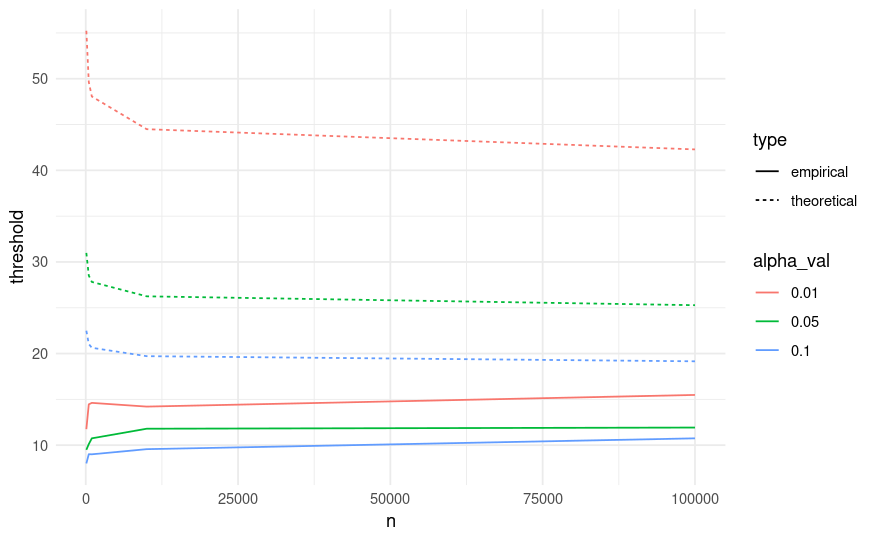
\includegraphics{source_imgs/empirical_thres_comparison.png}

We will see how to obtain this thresholds in the Lab.

\section{The Likelihood Ratio Test}\label{the-likelihood-ratio-test}

The CUSUM can be viewed as a special case of a more general framework
based on the Likelihood Ratio Test (LRT). This allow us to test for more
general settings, beyond simply detecting changes in the mean.

In general, the Likelihood Ratio Test is a method for comparing two
nested models: one under the null hypothesis, which assumes no
changepoint, and one under the alternative hypothesis, which assumes a
changepoint exists at some unknown position \(\tau\).

Suppose we have a set of observations \(x_1, x_2, \dots, x_n\). Under
the null hypothesis \(H_0\), we assume that all the data is generated by
the same model without a changepoint. Under the alternative hypothesis
\(H_1\), there is a single changepoint at \(\tau\), such that the model
for the data changes after \(\tau\). The LRT statistic is given by:

\begin{equation}\phantomsection\label{eq-lr-test}{
LR_\tau = - 2 \log \left\{ \frac{\max_{\theta} \prod_{t=1}^n L(y_{t}| \theta)}{\max_{\theta_1, \theta_2} [(\prod_{t=1}^n L(y_{t}| \theta_1))(\prod_{t=1}^n L(y_{t}| \theta_2)]} \right\}
}\end{equation}

The LRT compares the likelihood of the data under two models to
determine which one is more likely: the enumerator, is the likelihood
under the null hypothesis of no changepoint, while the denominator
represents the likelihood of the data under the alternative hypothesis,
where we optimise for two different parameters before and after the
changepoint at \(\tau\).

\subsection{Example: Gaussian
change-in-mean}\label{example-gaussian-change-in-mean}

The CUSUM statistics, in fact, is nothing but a specific case of this
model. To see this, we start from our piecewise costant signal, plus
noise, \(x_i = f_i + \epsilon_i, \quad i = 1, \dots, n\). Under this
model our data, a linear combination of a Gaussian, is distributed as:

\[
y_{i} \sim N(\mu_i, \sigma^2), \quad i = 1, \dots, n
\]

Therefore, to obtain the likelihood ratio test statistic, we plug our
Gaussian kernel into the LR above, and take the logarithm:

\[
LR_\tau = -2 \left[ \max_{\mu} \left( -\frac{1}{2\sigma^2} \sum_{i=1}^n (y_i - \mu)^2 \right) - \max_{\mu_1, \mu_2} \left( -\frac{1}{2\sigma^2} \left( \sum_{i=1}^\tau (y_i - \mu_1)^2 + \sum_{i=\tau+1}^n (y_i - \mu_2)^2 \right) \right)  \right]
\]

This simplifies to:

\[
= \frac{1}{\sigma^2} \left[ \min_{\mu} \sum_{i=1}^n (y_i - \mu_1)^2 - \min_{\mu_1, \mu_2} \left( \sum_{i=1}^\tau (y_i - \mu_1)^2 + \sum_{i=\tau+1}^n (y_i - \mu_2)^2 \right) \right]
\]

To solve the minimization over \(\mu_1\) and \(\mu_2\), we plug-in
values \(\hat\mu = \bar{y}_{1:n}\) on the first term, and
\(\hat\mu_1 = \bar{y}_{1:\tau}\), \(\hat\mu_2 = \bar{y}_{(\tau+1):n}\)
for the second term:

\[
LR_\tau = \frac{1}{\sigma^2} \left[ \sum_{i=1}^n (y_i - \bar{y}_{1:n})^2 - \sum_{i=1}^\tau (y_i - \bar{y}_{1:\tau})^2 - \sum_{i=\tau+1}^n (y_i - \bar{y}_{(\tau+1):n})^2 \right]
\]

This is the likelihood ratio test statistic for a change in mean in a
Gaussian model, which is essentially the CUSUM statistics squared,
rescaled by the known variance:

\[
LR_\tau = \frac{C_\tau^2}{\sigma^2}
\]

This is possible to prove directly with some tedious computations.

\textbf{Proof}. We start by writing down \(\sigma^2 LR\). This will be:

\[
\sigma^2 LR_\tau = \sum_{i=1}^{n} (y_i - \bar{y}_{1:n})^2 - \sum_{i=1}^{\tau} (y_i - \bar{y}_{1:\tau})^2 - \sum_{i=\tau+1}^{n} (y_i - \bar{y}_{\tau+1:n})^2
\]

Now we need to expand each term. Starting with the first:

\[
\sum_{i=1}^{n} (y_i - \bar{y}_{1:n})^2 = \sum_{i=1}^{n} y_i^2  - 2 \bar{y}_{1:n} \sum_{i=1}^{n} y_i + n \bar{y}_{1:n}^2 
\]

As \(\sum_{i=1}^{n} y_i = n \bar{y}_{1:n}\), we notice that we can
simplify the last two terms. We are left with:

\[
\sum_{i=1}^{n} (y_i - \bar{y}_{1:n})^2 = \sum_{i=1}^{n} y_i^2 - n \bar{y}_{1:\tau}^2
\]

We proceed similarly for the other two terms:

\[
\sum_{i=1}^{\tau} (y_i - \bar{y}_{1:\tau})^2 = \sum_{i=1}^{\tau} y_i^2 - \tau \bar{y}_{1:\tau}^2, \quad \sum_{i=\tau + 1}^{n} (y_i - \bar{y}_{\tau+1:n})^2 = \sum_{i=\tau+1}^{n} y_i^2 - (n-\tau) \bar{y}_{\tau+1:n}^2
\]

Putting all together, and getting rid of telescopic sums, we are left
with:

\[
\sigma^2 LR_\tau = - n \bar{y}_{1:n}^2 + \tau \bar{y}_{1:\tau}^2 + (n - \tau) \bar{y}_{\tau+1:n}^2.
\] Now, recall that
\(\bar{y}_{1:n} = \frac{1}{n} \left[ \tau \bar{y}_{1:\tau} + (n - \tau) \bar{y}_{\tau+1:n} \right]\),
and:

\[
\bar{y}_{1:n}^2 = \frac{1}{n^2}  \left[ \tau^2 \bar{y}_{1:\tau}^2 + 2 \tau (n - \tau) \bar{y}_{1:\tau}\bar{y}_{\tau+1:n} + (n - \tau)^2 \bar{y}_{\tau+1:n}^2 \right]
\]

Plugging in this into our LR:

\[
\begin{align}
\sigma^2 LR_\tau &= - \frac{\tau^2}{n} \bar{y}_{1:\tau}^2 - \frac{2 \tau (n - \tau)}{n} \bar{y}_{1:\tau}\bar{y}_{\tau+1:n}  - \frac{(n - \tau)^2}{n} \bar{y}_{\tau+1:n}^2 - \tau \bar{y}_{1:\tau}^2 - (n - \tau) \bar{y}_{\tau+1:n}^2=\\
&=  \frac{\tau (n - \tau)}{n} \bar{y}_{1:\tau}^2 -  \frac{2 \tau (n - \tau)}{n} \bar{y}_{1:\tau}\bar{y}_{\tau+1:n} + \frac{\tau (n - \tau)}{n}  \bar{y}_{\tau+1:n}^2 = \\  
&= \frac{\tau (n - \tau)}{n} (\bar{y}_{1:\tau}^2  - 2 \bar{y}_{1:\tau}\bar{y}_{\tau+1:n} + \bar{y}_{\tau+1:n}^2)=\\
&= \frac{\tau (n - \tau)}{n} (\bar{y}_{1:\tau} - \bar{y}_{\tau+1:n})^2=\\
&= C_\tau^2
\end{align}
\]

This gives us \(LR_\tau = \frac{C_\tau^2}{\sigma^2}\).

\section{Towards More General Models}\label{towards-more-general-models}

The great thing of the LR test is that it's extremely flexible, allowing
us to detect other changes then the simple change-in-mean case. As
before, the procedure is to compute the LR test conditional on a fixed
location of a changepoint, e.g.~\(LR_\tau\), and range across all
possible values for \(\tau\) to find the test statistics for our change.

\subsection{Change-in-variance}\label{change-in-variance}

To this end we will demostrate how to construct a test for Gaussian
change-in-variance, for mean known. For simplicy, we will call our
variance \(\sigma^2 = \theta\), our parameter of interest, and without
loss of generality, we can center our data on zero (e.g.~if
\(x_t \sim N(\mu, \theta)\), then
\(x_t - \mu = y_t \sim N(0, \theta)\)). Then, our p.d.f for one
observation will be given by:

\[
L(y_t | \theta) = \frac{1}{\theta \sqrt{2\pi}} \exp\{-\frac{y_t}{2 \theta}\}.
\] Plugging in the main LR test formula, we find:

\[
LR_\tau = - 2 \log \left\{ \frac{\max_{\theta} \prod_{t=1}^n \frac{1}{\theta \sqrt{2\pi}} \exp\{-\frac{y_t}{2 \theta}\}}{\max_{\theta_1, \theta_2} [(\prod_{t=1}^\tau \frac{1}{\theta \sqrt{2\pi}} \exp\{-\frac{y_t}{2 \theta}\})(\prod_{t=\tau+1}^n  \frac{1}{\theta \sqrt{2\pi}} \exp\{-\frac{y_t}{2 \theta}\}]} \right\}
\]

And taking the log, and simplifying over the constant gives us:

\[
\begin{align}
LR_\tau &= -\max_\theta \sum_{t = 1}^n \left(- \log(\theta) - \frac{y^2}{\theta} \right) + \max_{\theta_1, \theta_2}  \left[ \ \sum_{t = 1}^\tau \left( - \log(\theta_1) - \frac{y^2}{\theta_1} \right) + \sum_{t = \tau+1}^n \left(  - \log(\theta_2) - \frac{y^2}{\theta_2} \right) \right] = \\
& = -\min_\theta \sum_{t = 1}^n \left( \log(\theta) + \frac{y^2}{\theta} \right) + \min_{\theta_1, \theta_2}  \left[ \ \sum_{t = 1}^\tau \left(  \log(\theta_1) + \frac{y^2}{\theta_1} \right) + \sum_{t = \tau+1}^n \left(   \log(\theta_2) + \frac{y^2}{\theta_2} \right) \right]
\end{align}
\]

Now to solve the minimisation, we focus on the first term:

\[
f(y_{1:n}, \theta) = \sum_{t = 1}^n \left(  \log(\theta) + \frac{y^2}{\theta} \right) = \left(  n \log(\theta) + \frac{\sum_{t = 1}^n y^2}{\theta} \right).
\]

Taking the derivative with respect to \(\theta\), gives:

\[
\frac{d}{d\theta} f(y_{1:n}, \theta) = \frac{n}{\theta} - \frac{\sum_{t = 1}^n y^2}{\theta^2}
\] Setting equal to zero and solving for \(\theta\):

\[
n \theta - \sum_{t = 1}^n y^2 = 0
\]

Which gives us:
\(\hat\theta = \frac{\sum_{t = 1}^n y^2}{n} = \bar S_{1:n}\) the sample
variance.

Solving the optimization for \(\theta_1\) and \(\theta_2\) similarly,
gives us the values
\(\hat \theta_1 = \bar S_{1:\tau}, \ \hat \theta_2 = \bar S_{(\tau+1):n}\).

Now, as \(f(y_{1:n}, \hat{\theta}) = \bar S_{1:n} + n\) (why?) the final
LR test simplifies to:

\[
LR_\tau = \left[  - n \log(\bar S_{1:n}) + \tau \log(\bar S_{1:\tau}) + (n - \tau) \log(\bar S_{(\tau + 1):n}) \right]
\]

\includegraphics{2_control_files/figure-pdf/unnamed-chunk-3-1.pdf}

\subsection{Change-in-slope}\label{change-in-slope}

Another important exaple, and an alternative to detecting a
change-in-mean, is detecting a change in slope. In this section, we
assume the data is still modeled as a signal plus noise, but the signal
itself is a linear function of time (e.g.~non-stationary, with a
change!). Graphically:

\includegraphics{2_control_files/figure-pdf/unnamed-chunk-4-1.pdf}

More formally, let our data be modeled as:

\[
y_t = f_t + \epsilon_t, \quad t = 1, \dots, n,
\]

where the noise vector \(\epsilon_{1:n} \sim N(0, 1)\) consists of
independent and identically distributed (i.i.d.) normal random
variables. In this scenario, for simplicity, we assume a known constant
variance, which without loss of generality, we take to be 1.

Under the null hypothesis \(H_0\), we assume that the signal is linear
with a constant slope over the entire sequence, i.e.,

\[
f_t = \theta_0 + t\theta_1, \quad t = 1, \dots, n,
\]

where \(\theta_0\) is the intercept, and \(\theta_1\) is the slope.
However, under the alternative hypothesis \(H_1\), we assume there is a
changepoint at \(\tau\) after which the slope changes. Thus, the signal
becomes:

\[
f_t = \theta_0 + t\theta_1, \quad t = 1, \dots, \tau; \quad f_t = \theta_0 + \tau \theta_1 + (t-\tau)\theta_2, \quad t = \tau+1, \dots, n,
\]

where \(\theta_2\) is the new slope after the changepoint. In other
words, the model is showing a continuoos piecewise linear mean.

For this model, the log-likelihood ratio test statistic can be written
as the square of a projection of the data onto a vector \(v_\tau\),
i.e.,

\[
LR_\tau = \left( v_\tau^\top y_{1:n} \right)^2,
\]

where \(v_\tau\) is a contrast vector that is piecewise linear with a
change in slope at \(\tau\). This vector is constructed such that, under
the null hypothesis, the vector \(v_\tau^\top y_{1:n}\) has variance 1,
and \$ v\_\tau\^{}\top y\_\{1:n\}\$ is invariant to adding a linear
function to the data. These properties uniquely define the contrast
vector \(v_\tau\), up to an arbitrary sign. Computations on how to
obtain this likelihood ration test, and how to construct this vector are
beyond the scope of this module, but should you be curious those are
detailed in Baranowski, Chen, and Fryzlewicz (2019).

\subsection{Revisiting our Simpsons data
(again!)}\label{revisiting-our-simpsons-data-again}

So, going back to the Simpsons example\ldots{} We mentioned how the
belowed show rose rapidly to success, and at one point, started to
\emph{decline\ldots{}} A much better model would therefore be our
change-in-slope model!

To run the model, we can take advantage of the \texttt{not} package,
which by default is a multiple changepoint algorithm (we will see these
in the next week), but whose simplest case implements exactly our
change-in-slope LR test.

Before we proceed, we need to load, clean and standardize our data:

\begin{Shaded}
\begin{Highlighting}[]
\CommentTok{\# Load Simpsons ratings data}
\NormalTok{simpsons\_episodes }\OtherTok{\textless{}{-}} \FunctionTok{read.csv}\NormalTok{(}\StringTok{"extra/simpsons\_episodes.csv"}\NormalTok{)}
\NormalTok{simpsons\_episodes }\OtherTok{\textless{}{-}}\NormalTok{ simpsons\_episodes }\SpecialCharTok{|\textgreater{}} 
  \FunctionTok{mutate}\NormalTok{(}\AttributeTok{Episode =}\NormalTok{ id }\SpecialCharTok{+} \DecValTok{1}\NormalTok{, }\AttributeTok{Season =} \FunctionTok{as.factor}\NormalTok{(season), }\AttributeTok{Rating =}\NormalTok{ tmdb\_rating)}
\NormalTok{simpsons\_episodes }\OtherTok{\textless{}{-}}\NormalTok{ simpsons\_episodes[}\SpecialCharTok{{-}}\FunctionTok{nrow}\NormalTok{(simpsons\_episodes), ]}

\NormalTok{y }\OtherTok{\textless{}{-}}\NormalTok{ simpsons\_episodes}\SpecialCharTok{$}\NormalTok{Rating}
\end{Highlighting}
\end{Shaded}

We can then run our model with:

\begin{Shaded}
\begin{Highlighting}[]
\FunctionTok{library}\NormalTok{(not)}

\NormalTok{r }\OtherTok{\textless{}{-}} \FunctionTok{not}\NormalTok{(y, }\AttributeTok{method =} \StringTok{"max"}\NormalTok{, }\AttributeTok{rand.intervals =} \ConstantTok{FALSE}\NormalTok{, }\AttributeTok{contrast =} \StringTok{"pcwsLinContMean"}\NormalTok{, }\AttributeTok{intervals =} \FunctionTok{random.intervals}\NormalTok{(n, }\DecValTok{1}\NormalTok{, }\AttributeTok{min.length =}\NormalTok{ (n}\DecValTok{{-}1}\NormalTok{)))}

\FunctionTok{print}\NormalTok{(}\FunctionTok{paste0}\NormalTok{(}\StringTok{"Our changepoint estimate: "}\NormalTok{,  }\FunctionTok{features}\NormalTok{(r)}\SpecialCharTok{$}\NormalTok{cpt))}
\end{Highlighting}
\end{Shaded}

\begin{verbatim}
[1] "Our changepoint estimate: NA"
\end{verbatim}

\begin{Shaded}
\begin{Highlighting}[]
\FunctionTok{plot}\NormalTok{(r)}
\end{Highlighting}
\end{Shaded}

\includegraphics{2_control_files/figure-pdf/unnamed-chunk-6-1.pdf}

We notice how the test statistics implemented does not detect any
significant change\ldots{} As this may sound a bit anti-climatic, there
is still some relaxation on the hypotheses that we can do to obtain a
better answer. We can, in fact, relax the hypothesis that the regression
line needs to be continuous, and assume that there might be a change in
the intercept too, signifying an abrupt change:

\[
f_t = \theta_0 + t\theta_1, \quad t = 1, \dots, \tau; \quad f_t = \theta_0 + \theta_2 + \tau \theta_1 + (t-\tau)\theta_3, \quad t = \tau+1, \dots, n,
\]

We can do that by changing the model via the \texttt{contrast} argument:

\begin{Shaded}
\begin{Highlighting}[]
\NormalTok{r }\OtherTok{\textless{}{-}} \FunctionTok{not}\NormalTok{(y, }\AttributeTok{method =} \StringTok{"max"}\NormalTok{, }\AttributeTok{rand.intervals =} \ConstantTok{FALSE}\NormalTok{, }\AttributeTok{contrast =} \StringTok{"pcwsLinMean"}\NormalTok{, }\AttributeTok{intervals =} \FunctionTok{random.intervals}\NormalTok{(n, }\DecValTok{1}\NormalTok{, }\AttributeTok{min.length =}\NormalTok{ (n}\DecValTok{{-}1}\NormalTok{)))}

\FunctionTok{print}\NormalTok{(}\FunctionTok{paste0}\NormalTok{(}\StringTok{"Our changepoint estimate: "}\NormalTok{,  }\FunctionTok{features}\NormalTok{(r)}\SpecialCharTok{$}\NormalTok{cpt))}
\end{Highlighting}
\end{Shaded}

\begin{verbatim}
[1] "Our changepoint estimate: 176"
\end{verbatim}

\begin{Shaded}
\begin{Highlighting}[]
\FunctionTok{plot}\NormalTok{(r)}
\end{Highlighting}
\end{Shaded}

\includegraphics{2_control_files/figure-pdf/unnamed-chunk-7-1.pdf}

We can see that we now find a significant changepoint prior to episode
The Simpsons Spin-Off Showcase, which is anthology episode well over
into season 8, which is by many considered the last good one!

\section{Exercises}\label{exercises-1}

\subsection{Workshop 2}\label{workshop-2}

\begin{enumerate}
\def\labelenumi{\arabic{enumi}.}
\tightlist
\item
  Compute the LR ratio to detect a change in the success probability of
  a Bernoulli Random Variable.
\end{enumerate}

\subsection{Lab 2}\label{lab-2}

\begin{enumerate}
\def\labelenumi{\arabic{enumi}.}
\item
  Write a function, that taking as input \(n\) and a desired \(\alpha\)
  level for false positive rate, returns the threshold for the cusum
  statistics.
\item
  Construct a function that, taking as input \(n\), a desired \(\alpha\)
  , and a \texttt{replicates} parameter, runs a Monte Carlo simulation
  to tune an empirical penalty for the CUSUM change-in-mean on a simple
  Gaussian signal. Tip: You can reuse the function for computing the
  CUSUM statistics that you built the last week
\item
  Compare for a range of increasingly values of n,
  e.g.~\(n = 100, 500, 1000, 10.000\), and for few desired levels of
  alpha, the Monte Carlo threshold with the theoretically justified
  threshold. Plot the results, to recreate the plot above.
\item
  Using the Test the Simpsons dataset, find a critical level for your
  CUSUM statistics, and declare a change with the change-in-mean model.
\end{enumerate}

\bookmarksetup{startatroot}

\chapter{Multiple changepoints}\label{multiple-changepoints}

\section{Introduction}\label{introduction}

In real-world data, it is common to encounter situations where more than
one change occurs. When applying the CUSUM statistic in such cases,
where there are \textbf{multiple changes}, the question arises: how does
CUSUM behave, and how can we detect these multiple changes effectively?

\subsection{Real Example: Genomic Data and
Neuroblastoma}\label{real-example-genomic-data-and-neuroblastoma}

To motivate this discussion, we return to the example from week 1:
detecting active genomic regions using \emph{ChIP-seq data}. Our goal
here is to identify copy number variations (CNVs)---structural changes
in the genome where DNA sections are duplicated or deleted. These
variations can impact gene expression and are linked to diseases like
cancer, including neuroblastoma. The dataset we'll examine consists of
logratios of genomic probe intensities, which help us detect changes in
the underlying DNA structure.

Statistically our objective is to segment this logratio sequence into
regions with different means, corresponding to different genomic states:

\includegraphics{3_multiple_changes_files/figure-pdf/unnamed-chunk-2-1.pdf}

As seen from the plot, the data is noisy, but there are visible shifts
in the logratio values, suggesting multiple changes in the underlying
copy number. By the end of this chapter, we will segment this sequence!

\subsection{Towards multiple changes}\label{towards-multiple-changes}

Under this framework, the observed sequence \(y_t\) can be modeled as a
piecewise constant signal with changes in the mean occurring at each
changepoint \(\tau_k\). A plausible model for the change-in-mean signal
is given by

\[
y_t = \mu_k + \epsilon_t, \quad \text{for} \ \tau_k \leq t < \tau_{k+1}, \ k = 0, 1, \dots, K,
\]

where \(\mu_k\) is the mean of the \(k\)-th segment, and
\(\epsilon_t \sim \mathcal{N}(0, \sigma^2)\) are independent Gaussian
noise terms with mean 0 and (known) variance \(\sigma^2\).

As a starting example, we can generate a sequence with 4 segments, with
\(\tau_1 = 50, \tau_2 = 100, \tau_3 = 150\) and means
\(\mu_1 = 2, \mu_2 = 0, \mu_3 = -1\) and \(\mu_4 = 2\). Running the
CUSUM statistic in this scenario with multiple changes, leads to the
following \(C_\tau^2\) trace:

\includegraphics{3_multiple_changes_files/figure-pdf/unnamed-chunk-3-1.pdf}

From this, we notice that our test still has power to detect some of the
changes, but the estimate that we get, is initially wrong.
\(\Delta \mu = |\mu_1 - \mu_2|\). Is power lost when there is more then
one change in our test?

Well, to answer this question, we can compare the values of the CUSUM
statistic ran on the whole dataset (as above), with the values of the
CUSUM, ran on a subset containing only one change:

\begin{verbatim}
Warning: Removed 199 rows containing missing values or values outside the scale range
(`geom_line()`).
\end{verbatim}

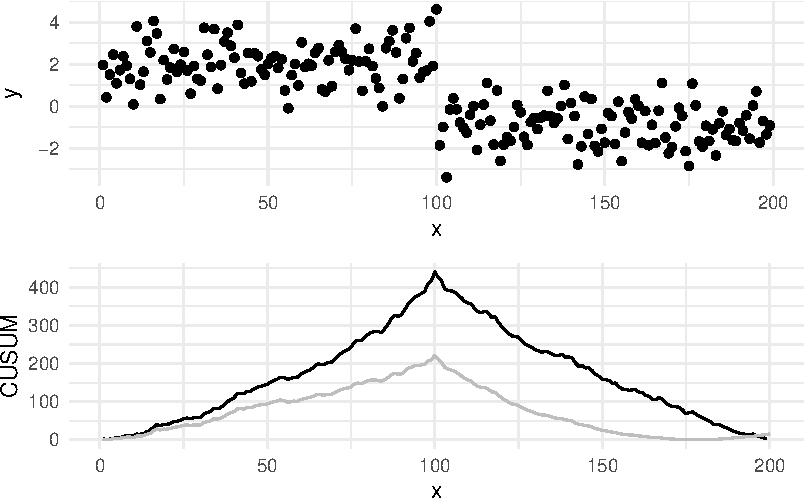
\includegraphics{3_multiple_changes_files/figure-pdf/unnamed-chunk-4-1.pdf}

We can see that max of the old cusum (the line in grey) is much lower
than the one where we isolate the sequence on one single change! So
there is an effective loss of power in this scenario in analyzing all
changes together, as some changes are masking the effects of
others\ldots{}

This gives us motivation to move towards some methodology that tries to
estimate all changes locations jointly, rather then one at a time!

\subsection{The cost of a
segmentation}\label{the-cost-of-a-segmentation}

Well, so far we only worked with one scheme that tried to split a
sequence in a hald

But how can we work in case we have more than one change? Well, we need
to introduce the cost of a segment.

If we assume the data is independent and identically distributed within
each segment, for segment parameter \(\theta\), then this cost can be
obtained through:

\[
    \mathcal{L}(y_{s+1:t}) = \min_\theta \sum_{i = s + 1}^{t} - \log(f(y_i, \theta))
\]

with \(f(y, \theta)\) being the likelihood for data point \(y\) if the
segment parameter is \(\theta\). Now, for example, in the gaussian case
this cost is given by:

\[
\mathcal{L}(y_{s:t}) = \frac{1}{2\sigma^2}  \sum_{i = s}^{t} \left ( y_i - \bar{y}_{s:t} \right)^2
\]

The cost for the full segmentation will be given by the sum across all
segments:

\[
\sum_{k = 0}^K \mathcal{L}(y_{\tau_k+1:\tau_{k+1}})
\]

Interestingly, the cost of a full segmentation is closely related to the
LR test. Consider, a single Gaussian change-in-mean at time \(\tau\),
splitting the data into two segments: \(y_{1:\tau}\) and
\(y_{\tau+1:n}\). The cost of this segmentation is:

\[
\mathcal{L}(y_{1:\tau}) + \mathcal{L}(y_{\tau+1:n}) = \frac{1}{\sigma^2} \left[\sum_{i=1}^{\tau} (y_i - \bar{y}_{1:\tau})^2 + \sum_{i=\tau+1}^{n} (y_i - \bar{y}_{(\tau+1):n})^2 \right]
\]

Which is essentially the same LR test as we saw last week, without the
null component. Specifically, for one change, minimizing the
segmentation cost over all possible changepoints locations \(\tau\) is
equivalent to maximizing the CUSUM statistic.

\subsection{The ``best'' segmentation}\label{the-best-segmentation}

We now have a way of evaluating how ``good'' a segmentation is, so it's
only natural to ask the question: what would be the best one?

Well, one way would be to, say, finding the the best set of
\(\tau = \tau_0, \dots, \tau_{K+1}\) changepoints that minimise the
cost:

\begin{equation}\phantomsection\label{eq-segment_cost}{
\min_{\substack{K \in \mathbb{N}\\ \tau_1, \dots, \tau_K}} \sum_{k = 0}^K \mathcal{L}(y_{\tau_k+1:\tau_{k+1}}).
}\end{equation}

Which one would this be? Say that for instance we range the
\(K = 1, \dots, n\), and at each step we find the best possible
segmentation. Graphically, we would be observing the following:

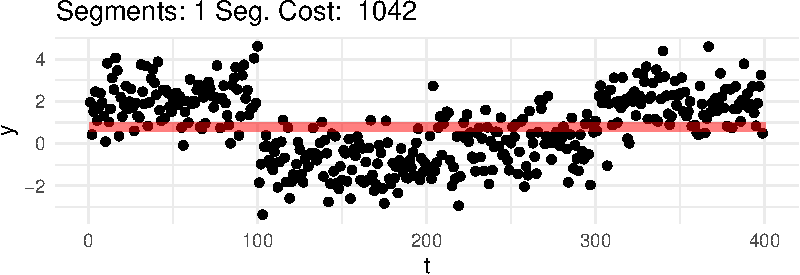
\includegraphics{3_multiple_changes_files/figure-pdf/unnamed-chunk-5-1.pdf}

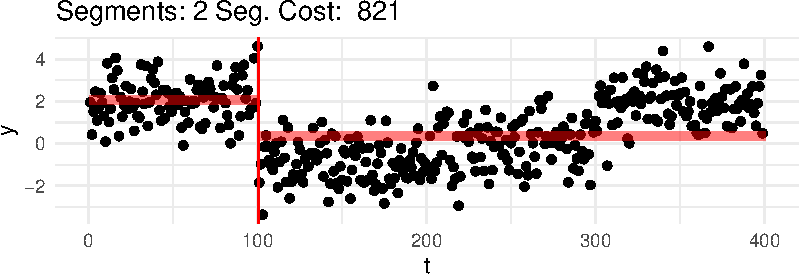
\includegraphics{3_multiple_changes_files/figure-pdf/unnamed-chunk-5-2.pdf}

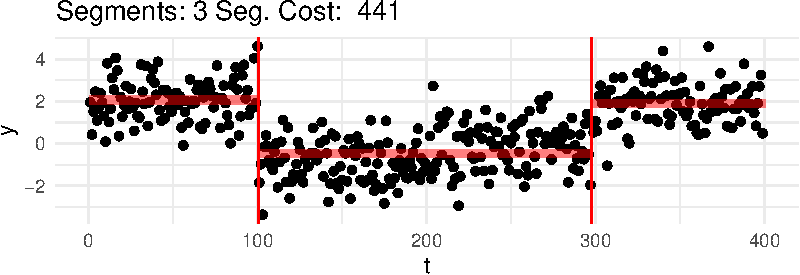
\includegraphics{3_multiple_changes_files/figure-pdf/unnamed-chunk-5-3.pdf}

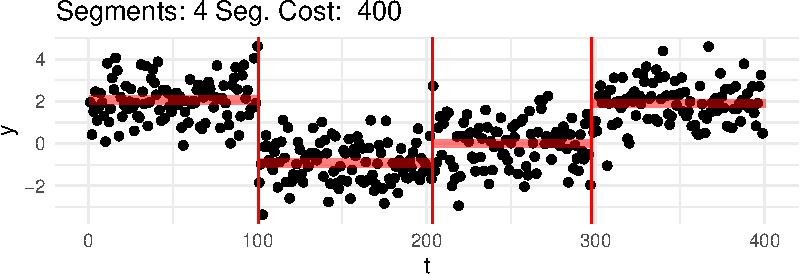
\includegraphics{3_multiple_changes_files/figure-pdf/unnamed-chunk-5-4.pdf}

Well, arguably we would like to stop at 4, which we know is the real
number of segments, but the cost keep going down\ldots{}

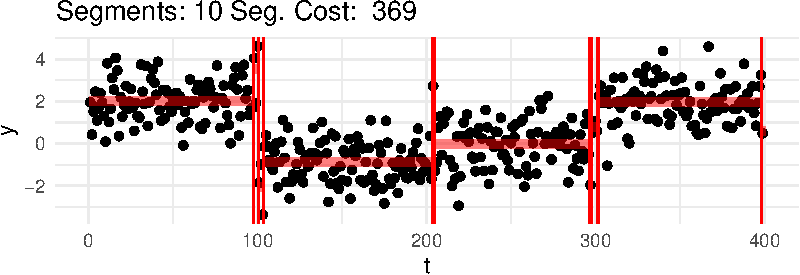
\includegraphics{3_multiple_changes_files/figure-pdf/unnamed-chunk-6-1.pdf}

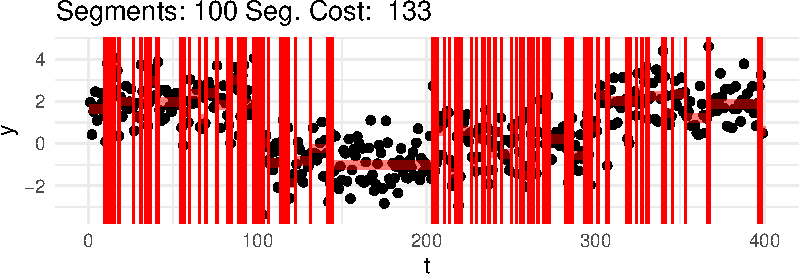
\includegraphics{3_multiple_changes_files/figure-pdf/unnamed-chunk-6-2.pdf}

And finally:

\includegraphics{3_multiple_changes_files/figure-pdf/unnamed-chunk-7-1.pdf}

\begin{center}

\includegraphics[width=5.0625in,height=\textheight]{source_imgs/fine.png}
\end{center}

Well, it turns out, that according to the minimization above, the
optimal segmentation across all would be the one that puts each point
into its own segment!

Well, there are different solutions to this problem. The first one we
will see, is a divide-and-conquer greedy approach, called Binary
Segmentation, and the second one will aim a generating a different
optimization to the one below that will find the optimal segmentation
\emph{up to a constant} to avoid over-fitting!

\section{Binary Segmentation}\label{binary-segmentation}

Binary Segmentation (BS) is a procedure from \cite{scott1974cluster} and
\cite{sen1975tests}. Binary segmentation works like this:

\begin{enumerate}
\def\labelenumi{\arabic{enumi}.}
\tightlist
\item
  Start with a test for a change \(\tau\) that splits a sequence into
  two segments and to check if the cost over those two segments, plus a
  penalty \(\beta \in \mathbb{R}\), is smaller then the cost computed on
  the whole sequence:
  \begin{equation}\phantomsection\label{eq-bin_seg_condition}{
      \mathcal{L}(y_{1:\tau}) + \mathcal{L}(y_{\tau+1:n}) + \beta < \mathcal{L}(y_{1:n})     
  }\end{equation}
\end{enumerate}

where the segment cost \(\mathcal{L}(\cdot)\), is as in
Equation~\ref{eq-segment_cost}.

\begin{enumerate}
\def\labelenumi{\arabic{enumi}.}
\setcounter{enumi}{1}
\item
  If the condition in Equation~\ref{eq-bin_seg_condition} is true for at
  least one \(\tau \in 1, \dots, n\), then the \(\tau\) that minimizes
  \(\mathcal{L}(y_{1:\tau}) + \mathcal{L}(y_{\tau+1:n})\) is picked as a
  first changepoint and the test is then performed on the two newly
  generated splits. This step is repeated until no further changepoints
  are detected on all resulting segments.
\item
  If there are no more resulting valid splits, then the procedure ends.
\end{enumerate}

Some of you might have noted how the condition in
Equation~\ref{eq-bin_seg_condition} is closely related to the LR test in
Equation~\ref{eq-lr-test}. In fact, rearranging equation above, gives
us:

\[
- \mathcal{L}(y_{1:n}) + \mathcal{L}(y_{1:\tau}) + \mathcal{L}(y_{\tau+1:n}) = - \frac{LR_\tau}{2}  < -\beta.
\]

The \(-\beta\) acts exactly as the constant \(c\) for declaring a
change, and it adds a natural stopping condition, solving the issue of
overfitting that we mentioned in the previous section! Binary
Segmentation, in fact, does nothing more then iteratively running a LR
test, until no changes are found anymore!

This gives us a strategy to essentially apply a test that is locally
optimal for one change, such as the Likelihood Ratio test, to solve a
multiple changepoint segmentation. For this reason, BS is often employed
to extend single changepoint procedures to multiple changes procedures,
and hence it is one of the most prominent methods in the literature.

\subsection{Binary Segmentation in
action}\label{binary-segmentation-in-action}

Having introduced the main idea, we show now how binary segmentation
works in action with an example above. Say that we set a
\(\beta = 2 \log(400) =\) 11.98.

\textbf{Step 1:} We start by computing the cost as in
Equation~\ref{eq-bin_seg_condition}, and for those that are less then
\(\beta\), we pick the smallest. This will be our first changepoint
estimate, and the first point of split.

In the plots below, the blue horizontal line is the mean signal
estimated for a given split, while in the cusum the pink will represent
the values of the LR below the threshold \(\beta\), and red vertical
line will show the min of the test statistics. When the cost is below
the beta line, this will be our changepoint estimate.

In our case, we can see that the min of our cost has been achieved for
\(\hat\tau=100\), and since this is below the threshold, it's our first
estimated changepoint!

\includegraphics{3_multiple_changes_files/figure-pdf/unnamed-chunk-8-1.pdf}

\textbf{Step 2:}

From the first step, we have to check now two splits:

\begin{itemize}
\item
  The first left split, \textbf{1-LEFT} in the plot below, covers data
  \(y_{1:100}\). We can see that from here, the min of our statistic is
  below the threshold, therefore we won't declare any further change in
  this subset.
\item
  The first right split, \textbf{1-RIGHT} covers data \(y_{101:400}\).
  We can see that here, the min of the statistics, is below the
  threshold, and therefore we identify a second change at
  \(\hat\tau = 297\). This is not exactly 300, so we don't have a
  perfect estimate. Despite this is not ideal, this is the best point we
  have found and therefore we have to continue!
\end{itemize}

\includegraphics{3_multiple_changes_files/figure-pdf/unnamed-chunk-9-1.pdf}

\textbf{Step 3:}

In step 3, we have to check again two splits splits:

\begin{itemize}
\item
  The second left split, \textbf{2-LEFT} in the plot below, covers data
  \(y_{101:297}\). Now, it's in this split that the statistics goes
  below the threshold! The third estimated change is at
  \(\hat\tau = 203\), again slightly off the real one at 200. We
  continue investigating this split\ldots{}
\item
  The second right split, \textbf{2-RIGHT} covers data \(y_{298:400}\).
  In this last split, the min is not over the threshold, therefore we
  stop the search.
\end{itemize}

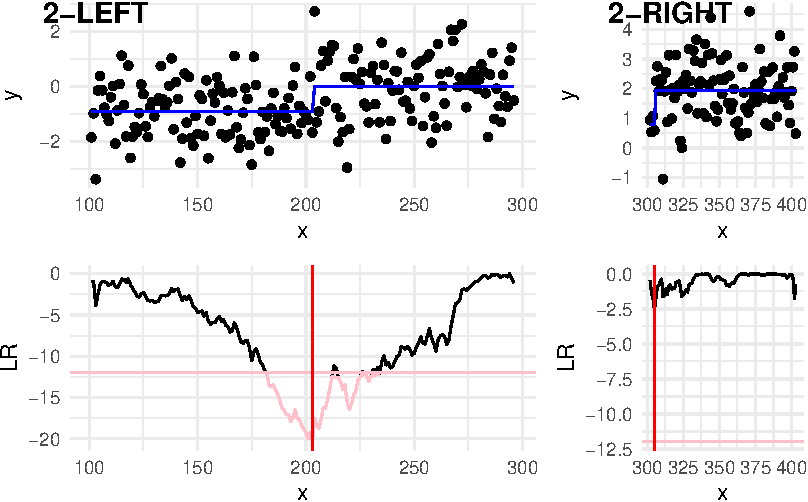
\includegraphics{3_multiple_changes_files/figure-pdf/unnamed-chunk-10-1.pdf}

\textbf{Step 4:}

In step 4, we check:

\begin{itemize}
\item
  The third left split, \textbf{3-LEFT} in the plot below, covers data
  \(y_{101:203}\). The minimum, in here is not over the threshold.
\item
  The third right split, \textbf{3-RIGHT} covers data \(y_{204:298}\).
  Similarly, the minimum is not over the treshold.
\end{itemize}

\includegraphics{3_multiple_changes_files/figure-pdf/unnamed-chunk-11-1.pdf}

The algorithm therefore terminates!

With this graphical description in mind, we formally describe the Binary
Segmentation algorithm as a recursive procedure, where the first
iteration would be simply given by \(\text{BinSeg}(y_{1:n}, \beta)\).

\begin{center}\rule{0.5\linewidth}{0.5pt}\end{center}

\(\text{BinSeg}(y_{s:t}, \beta)\)\\

\begin{center}\rule{0.5\linewidth}{0.5pt}\end{center}

\textbf{INPUT:} Subseries \(y_{s:t} = \{y_s, \dots, y_t\}\) of length
\(t - s + 1\), penalty \(\beta\)\\
\textbf{OUTPUT:} Set of detected changepoints \(cp\)\\
\strut \\
\textbf{IF} \(t - s \leq 1\)\\
\strut ~~~~\textbf{RETURN} \(\{\}\) // No changepoint in segments of
length 1 or less\\
\strut \\
\textbf{COMPUTE}\\
\(\mathcal{Q} \leftarrow \underset{\tau \in \{s, \dots, t\}}{\min} \left[ \mathcal{L}(y_{s:\tau}) + \mathcal{L}(y_{\tau+1:t}) - \mathcal{L}(y_{s:t}) + \beta \right]\)\\
\strut \\
\textbf{IF} \(\mathcal{Q} < 0\)\\
\strut ~~~~\(\hat{\tau} \leftarrow \underset{\tau \in \{s, \dots, t\}}{\text{arg}\min} \left[ \mathcal{L}(y_{s:\tau}) + \mathcal{L}(y_{\tau+1:t}) - \mathcal{L}(y_{s:t}) \right]\)\\
\strut ~~~~~\(cp \leftarrow \{ \hat{\tau}, \text{BinSeg}(y_{s:\hat{\tau}}, \beta), \text{BinSeg}(y_{\hat{\tau}+1:t}, \beta) + \hat\tau \}\)\\
\strut ~~~~~\textbf{RETURN} \(cp\)\\
\strut \\
\textbf{RETURN} \(\{\}\) // No changepoint if \(-LR/2\) is above penalty
\(- \beta\)

\begin{center}\rule{0.5\linewidth}{0.5pt}\end{center}

\section{Optimal Partitioning}\label{optimal-partitioning}

Another solution to avoid the over-fitting problem of
Equation~\ref{eq-segment_cost} lies in introducing a penalty term that
discourages too many changepoints, avoiding overfitting. This is known
as the \emph{penalised approach}.

To achieve this, we want to minimize the following cost function:

\begin{equation}\phantomsection\label{eq-pen-cost}{
Q_{n, \beta} = \min_{K \in \mathbb{N}} \left[ \min_{\substack{\\ \tau_1, \dots, \tau_K}} \sum_{k = 0}^K \mathcal{L}(y_{\tau_k+1:\tau_{k+1}}) + \beta K
 \right],
}\end{equation}

where \(Q_{n, \beta}\) represents the optimal cost for segmenting the
data up to time \(n\) with a penalty \$ \beta \$ that increases with
each additional changepoint \(K\). With the \(\beta\) term, for every
new changepoint added, the cost of the full segmentation increases,
discouraging therefore models with too many changepoints.

Unlike Binary Segmentation, which works iteratively and makes local
decisions about potential changepoints, and as we have seen it is prone
to errors, solving \(Q_{n, \beta}\) ensures that the segmentation is
\textbf{globally optimal}, as in the location of the changes are the
best possible to minimise our cost.

Now, directly solving this problem using a brute-force search is
computationally prohibitive, as it would require checking every possible
combination of changepoints across the sequence: the number of possible
segmentations grows exponentially as \(n\) increases\ldots{}

Fortunately, this problem can be solved efficiently using a sequential,
dynamic programming algorithm: \textbf{Optimal Partitioning (OP)}, from
Jackson et al. (2005). OP solves Equation~\ref{eq-pen-cost} exactly
through the following recursion.

We start with \(\mathcal{Q}_{0, \beta} = -\beta\), and then, for each
\(t = 1, \dots, n\), we compute:

\begin{equation}\phantomsection\label{eq-optimal-partitioning}{
    \mathcal{Q}_{t, \beta} = \min_{0 \leq \tau < t} \left[ \mathcal{Q}_{\tau, \beta} + \mathcal{L}(y_{\tau + 1:t}) + \beta \right].
}\end{equation}

Here, \(\mathcal{Q}_{t, \beta}\) represents the optimal cost of
segmenting the data up to time \(t\). The algorithm builds this solution
sequentially by considering each possible segmentation
\(\mathcal{Q}_{0, \beta},\ \cdots, \mathcal{Q}_{t-2, \beta},\ \mathcal{Q}_{t-1, \beta}\)
before the current time \(t\), plus the segment cost up to current time
\(t\), \(\mathcal{L}(y_{\tau + 1:t})\).

\subsection{Optimal partitinioning in
action}\label{optimal-partitinioning-in-action}

This recursion can be quite hard to digest, and is, as usual, best
described graphically.

\textbf{Step 1} Say we are at \(t = 1\). In this case, according to
equation above, the optimal cost up to time one will be given by
(remember that the \(\beta\) cancels out with \(Q_{0, \beta}\)!):

\[
 \mathcal{Q}_{1, \beta} = \left[ -\beta + \mathcal{L}(y_{1:1}) + \beta \right] = \mathcal{L}(y_{1:1})
\]

\includegraphics{3_multiple_changes_files/figure-pdf/unnamed-chunk-12-1.pdf}

\textbf{Step 2.} Now, at the second step, we have to minimise between
two segmentations:

\begin{itemize}
\tightlist
\item
  One with the whole sequence in a second segment alone (again,
  \(\beta\) cancels out with \(Q_{0, \beta} = -\beta\)), and this will
  be given by \(\mathcal{L}(y_{1:2})\) (dotted line)
\item
  One with the optimal segmentation from step 1
  \(\mathcal{Q}_{1, \beta}\) (whose cost considered only the first point
  in its own segment!), to which we have to sum the cost relative to a
  second segment \(\mathcal{L}(y_{2:2})\) that puts the second point
  alone, and the penalty \(\beta\) as we have added a new segment!
\end{itemize}

We minimise across the two, and this gives us \(Q_{2, \beta}\).

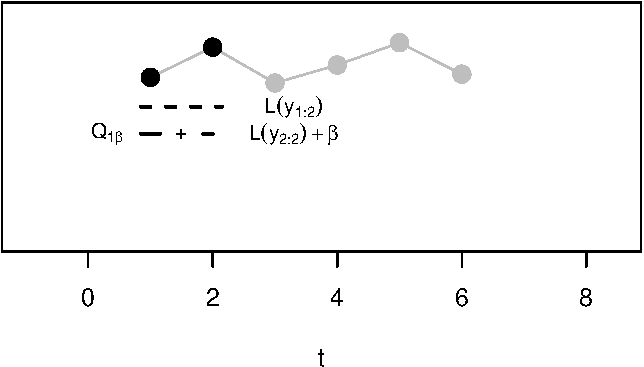
\includegraphics{3_multiple_changes_files/figure-pdf/unnamed-chunk-13-1.pdf}

\emph{Step 3}: Similarly, at \(t = 3\) we have now three segmentations
to choose from:

\begin{itemize}
\item
  The one that puts the first three observations in the same segment,
  whose cost will be given simply by \(\mathcal{L}(y_{1:2})\),
\item
  The one considering the optimal segmentation from time 1, plus the
  cost of adding an extra segment with observation 2 and 3 together
\item
  Finally the optimal from segmentation 2, \(\mathcal{Q}_{2, \beta}\),
  plus the segment cost of fitting an extra segment with point 3 alone.
  Note that \(\mathcal{Q}_{2, \beta}\) will come from the step before:
  if we would have been beneficial to add a change, at the previous
  step, this information is carried over!
\end{itemize}

Again, we pick the minimum across these three to get
\(\mathcal{Q}_{3, \beta}\), and proceed.

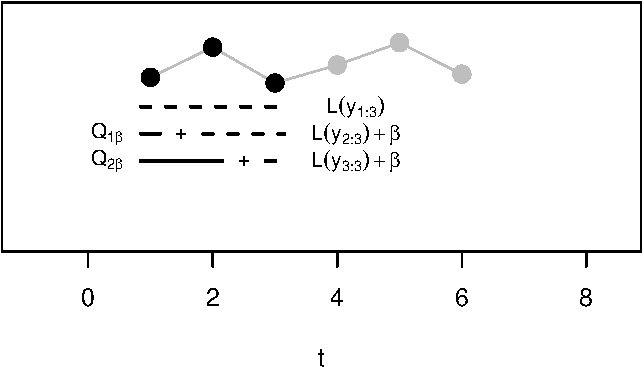
\includegraphics{3_multiple_changes_files/figure-pdf/unnamed-chunk-14-1.pdf}

\emph{Step} \(n\) Until the last step! Which would look something like
this:

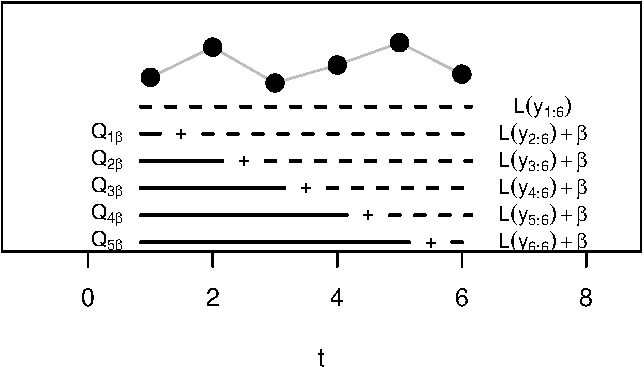
\includegraphics{3_multiple_changes_files/figure-pdf/unnamed-chunk-15-1.pdf}

A formal description of the algorithm can be found below:

\begin{center}\rule{0.5\linewidth}{0.5pt}\end{center}

\textbf{INPUT:} Time series \(y = (y_1, ..., y_n)\), penalty \(\beta\)\\
\textbf{OUTPUT:} Optimal changepoint vector \(cp_n\)\\
\strut \\
Initialize \(\mathcal{Q}_0 \leftarrow -\beta\)\\
Initialize \(cp_0 \leftarrow \{\}\)\\
\strut \\
\textbf{FOR} \(t = 1, \dots, n\)\\
\strut ~~~~~\(\mathcal{Q}_t \leftarrow \min_{0 \leq \tau < t} \left[ \mathcal{Q}_{\tau} + \mathcal{L}(y_{\tau + 1:t}) + \beta \right]\)\\
\strut ~~~~~\(\hat\tau \leftarrow \text{arg}\min_{0 \leq \tau < t} \left[ \mathcal{Q}_{\tau} + \mathcal{L}(y_{\tau + 1:t}) + \beta \right]\)\\
\strut ~~~~~\(cp_t \leftarrow (cp_{\hat\tau}, \hat\tau)\) // Append the
changepoint to the list at the last optimal point\\
\strut \\
\textbf{RETURN} \(cp_n\)

\begin{center}\rule{0.5\linewidth}{0.5pt}\end{center}

Running the Optimal Partitioning method on our example scenario, with
the same penalty \(\beta = 2 \log(400) =\) 11.98 as above, gives
changepoint locations \(\tau_{1:4} = \{100, 203, 301\}\).

\begin{verbatim}
Loading required package: zoo
\end{verbatim}

\begin{verbatim}

Attaching package: 'zoo'
\end{verbatim}

\begin{verbatim}
The following objects are masked from 'package:base':

    as.Date, as.Date.numeric
\end{verbatim}

\begin{verbatim}
Successfully loaded changepoint package version 2.2.4
 See NEWS for details of changes.
\end{verbatim}

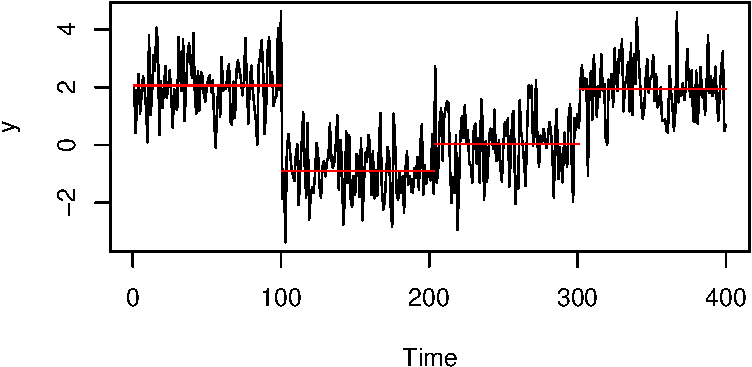
\includegraphics{3_multiple_changes_files/figure-pdf/unnamed-chunk-16-1.pdf}

So we can see how on this dataset in particular, OP performs slightly
better then Binary Segmentation on the last change, getting closer to
the real changepoint of 300!

\subsection{Neuroblastoma example}\label{neuroblastoma-example}

Returning to the original example at the start of the module, the
neuroblastoma dataset, we run both Binary Segmentation, and Optimal
Partitioning.

We report results in the plot below (blue for BS, green for OP). In this
case, the algorithms return the same four changepoints:

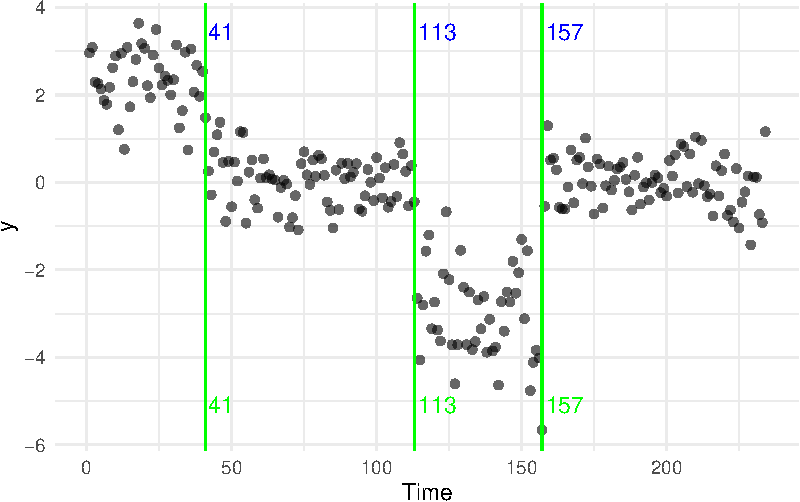
\includegraphics{3_multiple_changes_files/figure-pdf/unnamed-chunk-17-1.pdf}

Some of you might come up with two (very interesting) questions that
hopefully we will answer next week\ldots{}

\begin{itemize}
\item
  If the methods perform roughly the same, which one do I choose?
\item
  Why is the data on a different scale then that presented at the start
  of the chapter?
\end{itemize}

\section{Exercises}\label{exercises-2}

\subsection{Workshop 3}\label{workshop-3}

\begin{enumerate}
\def\labelenumi{\arabic{enumi}.}
\tightlist
\item
  For the vector \(y_{1:4} = (0.5, -0.1, 12.1, 12.4)\), and a penalty
  \(\beta = 5\) calculate, pen on paper (and calculator), all the Binary
  Segmentation, and Optimal Partitioning steps. \textbf{TIP}: To speed
  up computations, you want to pre-compute all segment costs
  \(\mathcal{L}(y_{l:u})\). I have pre-computed some of these costs in
  the table below:
\end{enumerate}

\[
\begin{array}{c|cccc}
l \backslash u & 1 & 2 & 3 & 4 \\
\hline
1 & \mathcal{L}(y_{1:1}) & 0.18 & 94.59 & 145.43 \\
2 &  & 0.00 & \mathcal{L}(y_{2:3}) & 101.73 \\
3 &  &  & 0.00 & \mathcal{L}(y_{3:4}) \\
4 &  &  &  & 0.00 \\
\end{array}
\]

\subsection{Lab 3}\label{lab-3}

\begin{enumerate}
\def\labelenumi{\arabic{enumi}.}
\item
  Code the Optimal Partitioning algorithm for the Gaussian
  change-in-mean case.\\
  \textbf{Tips:}

  \begin{enumerate}
  \def\labelenumii{\alph{enumii}.}
  \item
    Again, you can pre-compute all the possible
    \(\mathcal{L}(y_{l:u})\), for \(u \geq l\) to save computational
    time.
  \item
    Be very careful with indexing\ldots{} R starts indexing at 1,
    however, in the pseudocode, you have one element that starts at
    0\ldots{}
  \end{enumerate}
\item
  Install the \texttt{changepoint} package. The example signal of
  Section 3.4, with the same penalty value of \(\beta = 2 * log(n)\),
  compare your implementation of OP, Binary Segmentation, and PELT. You
  will learn how to do so in the documentation, running
  \texttt{?cpt\_mean}. You should make 300 replicates each of your
  experiment, and compare:

  \begin{enumerate}
  \def\labelenumii{\alph{enumii}.}
  \item
    The absolute error loss from the mean signal,
    e.g.~\(||\mu_{1:n} - \hat{\mu}_{1:n}||^2_2\)
  \item
    The absolute error in the number of changepoints reconstructed,
    e.g.~\(|K - \hat{K}|\). What do we observe?
  \item
    The runtime for one sequence of PELT agains Binary Segmentation.
    Evaluate the runtime with package \texttt{microbenchmark}.
  \end{enumerate}
\end{enumerate}

\bookmarksetup{startatroot}

\chapter{PELT, WBS and Penalty
choices}\label{pelt-wbs-and-penalty-choices}

\section{Drawbacks of OP and BS}\label{drawbacks-of-op-and-bs}

When deciding which segmentation approach to use, Binary Segmentation
(BS) and Optimal Partitioning (OP) each offer different strengths. The
choice largely depends on the characteristics of the data and the goal
of the analysis.

\subsection{Quality of the
Segmentation}\label{quality-of-the-segmentation}

Generally, Optimal Partitioning (OP) provides the \emph{most accurate
segmentation}, especially when we have a well-defined model and expect
precise changepoint detection. OP ensures that the solution is optimal
by globally minimizing the cost function across all possible
segmentations. This is ideal for datasets with clear changes, even if
noise is present.

Let's consider a case with true changepoints at
\(\tau = 100, 200, 300\), and segment means
\(\mu_{1:4} = 2, 1, -1, 1.5\):

\includegraphics{4_algos_and_penalties_files/figure-pdf/unnamed-chunk-2-1.pdf}

While the underlying signal follows these clear shifts, noise
complicates segmentation. Binary Segmentation uses a greedy process
where each iteration looks for the largest changepoint. Although fast,
this local search can make mistakes if the signal isn't perfectly clear,
particularly in the early stages of the algorithm. For example, running
BS on this dataset introduces a mistake at \(\tau = 136\), as shown in
the plot below:

\includegraphics{4_algos_and_penalties_files/figure-pdf/unnamed-chunk-3-1.pdf}

This error is carried in the subsequent steps, and the full binary
segmentation algorithm will output an additional change at
\(\tau = 136\)\ldots{} Optimal Partitioning (OP), on the other hand,
evaluates all possible segmentations considers the overall fit across
the entire sequence. It is therefore less susceptible to adding
``ghost'' changepoints, as rather than focusing on the largest change at
each step.

To illustrate, we compare the segmentations generated by both
approaches:

\includegraphics{4_algos_and_penalties_files/figure-pdf/unnamed-chunk-4-1.pdf}

\subsection{Computational Complexity}\label{computational-complexity}

Well, you may ask why not using OP all the time, then? Well, in
changepoint detection, in which is the most appropiate method, we often
have to keep track of the computational performance too, and Binary
Segmentation is faster on average. For this reason, for large datasets
where approximate solutions are acceptable, it might be the best option.

Specifically:

\begin{itemize}
\item
  \textbf{Binary Segmentation} starts by dividing the entire sequence
  into two parts, iteratively applying changepoint detection to each
  segment. In the average case, it runs in \(\mathcal{O}(n \log n)\)
  because it avoids searching every possible split point. However, in
  the worst case (if all data points are changepoints), the complexity
  can degrade to \(\mathcal{O}(n^2)\), as each step can require
  recalculating test statistics for a growing number of segments.
\item
  \textbf{Optimal Partitioning}, on the other hand, solves the
  changepoint problem by recursively considering every possible split
  point up to time \(t\). The result is an optimal segmentation, but at
  the cost of \(\mathcal{O}(n^2)\) computations. This holds true for
  both the average and worst cases, as it always requires a full
  exploration of all potential changepoints.
\end{itemize}

\section{PELT and WBS}\label{pelt-and-wbs}

Good news is, despite both algorithms have drawbacks, following
\emph{recent developments}, those have been solved. In the next
sections, we will introduce two new algorithms, PELT and WBS.

\subsection{PELT: an efficient solution to
OP}\label{pelt-an-efficient-solution-to-op}

In OP, we can reduce the numbers of checks to be performed at each
iteration, reducing the complexity. This operation is called
\emph{pruning}. Specifically, on the condition that there exists a
constant \(\kappa\) such that for every \(l < t < u\):

\[
        \mathcal{L}(y_{l + 1:t}) + \mathcal{L}(y_{t + 1:u}) + \kappa \leq \mathcal{L}(y_{l + 1:u})
\]

It is possible to \emph{prune} without resorting to an approximation.
For many cost functions, such as the Gaussian cost, such a constant
exists. Equating \(\kappa\) to the penalty \(\beta\), gives us a
computational trick to improve on the efficiency\ldots{} The PELT
algorithm -- acronym for Pruned Exact Linear Time -- (Killick,
Fearnhead, and Eckley (2012)) solves exactly the penalised minimization
of Equation~\ref{eq-optimal-partitioning} with an expected computational
cost that can be linear in \(n\) -- while still retaining
\(\mathcal{O}(n^2)\) computational complexity in the worst case. This is
achieved by reducing the number of segment costs to evaluate at each
iteration via an additional pruning step based on Condition
Equation~\ref{eq-optimal-partitioning}. That is, if
\[\mathcal{Q}\tau + \mathcal{L}(y_{\tau + 1:t}) + \kappa \geq \mathcal{Q}_t\]
then we can safely prune the segment cost related to \(\tau\), as
\(\tau\) will never be the optimal changepoint location up to any time
\(T > t\) in the future.

The intuition, is that, when \(\kappa = \beta\), our penalty, then we
would prune at every change detected. And if the changes increase
linearly with the length of the data, this means that our algorithm will
achieve a \(\mathcal{O}(n \log n)\) computational complexity, without
any drawbacks!

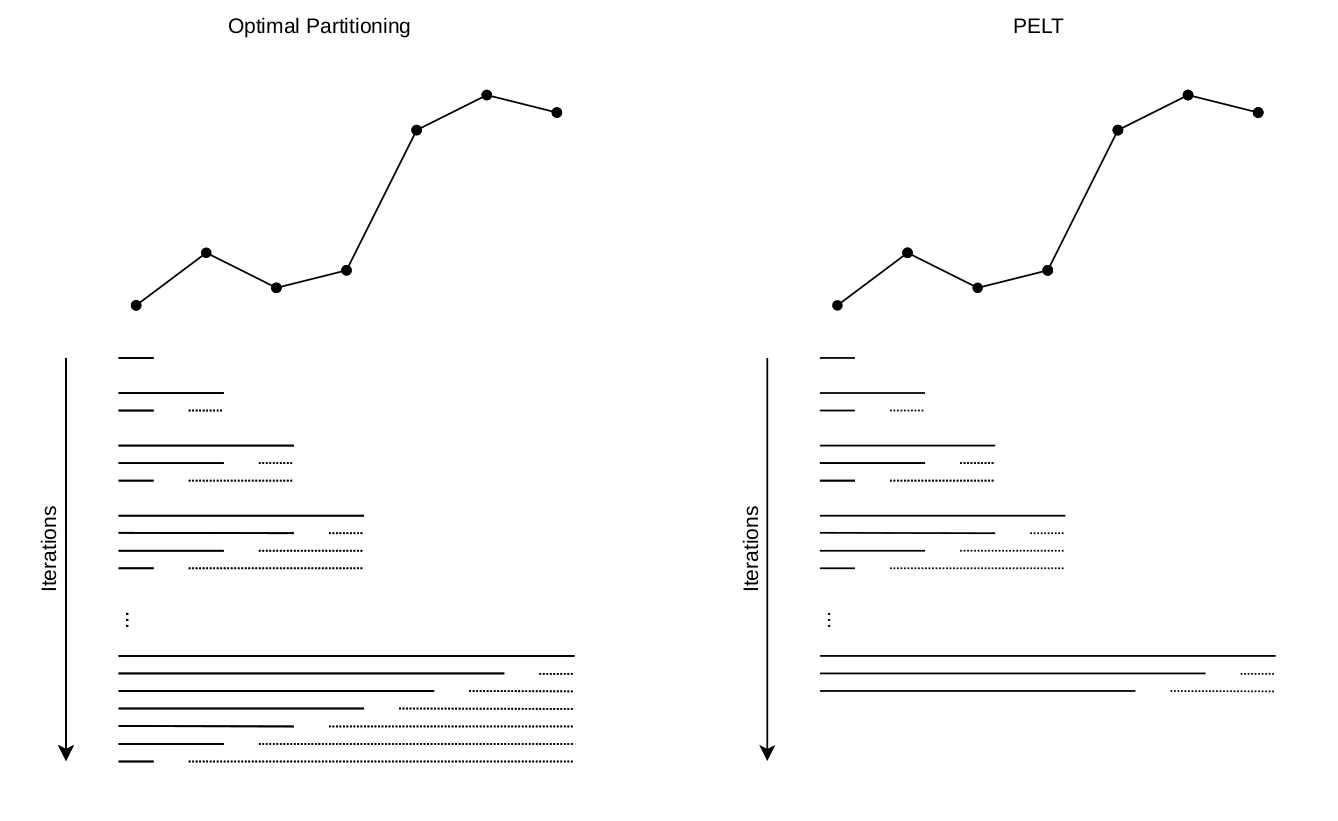
\includegraphics{source_imgs/OPPELT.png}

To reduce computational complexity, we can slightly modify the OP
algorithm, to add the pruning condition above:

\begin{longtable}[]{@{}l@{}}
\toprule\noalign{}
\endhead
\bottomrule\noalign{}
\endlastfoot
PELT \\
\end{longtable}

\textbf{INPUT:} Time series \(y = (y_1, ..., y_n)\), penalty \(\beta\)\\
\textbf{OUTPUT:} Optimal changepoint vector \(cp_n\)\\
\strut \\
Initialize \(\mathcal{Q}_0 \leftarrow -\beta\)\\
Initialize \(cp_0 \leftarrow \{\}\)\\
Initialise \(R_1 = \{0\}\)\\
\strut \\
\textbf{FOR} \(t = 1, \dots, n\)\\
\strut ~~~~~\(\mathcal{Q}_t \leftarrow \min_{\tau \in R_t} \left[ \mathcal{Q}_{\tau} + \mathcal{L}(y_{\tau + 1:t}) + \beta \right]\)\\
\strut ~~~~~\(\hat\tau \leftarrow \text{arg}\min_{\tau \in R_t} \left[ \mathcal{Q}_{\tau} + \mathcal{L}(y_{\tau + 1:t}) + \beta \right]\)\\
\strut ~~~~~\(cp_t \leftarrow (cp_{\hat\tau}, \hat\tau)\) // Append the
changepoint to the list at the last optimal point\\
\strut ~~~~~\(R_{t+1} \leftarrow \{\tau \in \{R_t \cup \{t\}\} : \mathcal{Q}_\tau + \mathcal{L}(y_{\tau + 1:t}) + \beta \leq \mathcal{Q}_t \}\)
// prune the non-optimal changepoint locations\\
\strut \\
\textbf{RETURN} \(cp_n\)

\begin{center}\rule{0.5\linewidth}{0.5pt}\end{center}

As the segmentation retained is effectively the same, there are
literally no disadvantages in using PELT over OP, if the cost function
allows to do so.

However, PELT still has some disadvantages:

\begin{itemize}
\item
  PELT pruning works only over some cost functions, those for which the
  condition above is true. For example, in the continuous
  change-in-slope case, we have that the cost from the next change
  depends on the location of the previous one, making it impossible for
  PELT to prune without loosing optimality.
\item
  We mentioned above how PELT over iterations at which a change is
  detected. For signals where changes are not frequent, PELT does not
  benefits from. A more sophisticated approach is that of \textbf{FPOP},
  that prunes at every iteration. FPOP employs a different type of
  pruning, called functional pruning, that at every iteration only check
  costs that are likely associated to a change. However, despite the
  pruning is stronger FPOP works only over few selected models.
\end{itemize}

\subsection{WBS: Improving on Binary
Segmentation}\label{wbs-improving-on-binary-segmentation}

In BS, one of the issues that may arise, is an incorrect segmentation.
WBS, Fryzlewicz (2014), is a multiple changepoints procedures that
improve on the BS changepoint estimation via computing the initial
segmentation cost of BS multiple times over \(M + 1\) random subsets of
the sequence, \(y_{s_1:t_1}, \dots, y_{s_M:t_M}, y_{1:n}\), picking the
best subset according to what achieves the smallest segmentation cost
and reiterating the procedure over that sample accordingly. The idea
behind WBS lies in the fact that a favorable subset of the data
\(y_{s_m:t_m}\) could be drawn which contains a true change sufficiently
separated from both sides \(s_m, t_m\) of the sequence. By the inclusion
of the \(y_{1:n}\) entire sequence among the subsets, it is guaranteed
that WBS will do no worse than the simple BS algorithm.

We can formally provide a description of WBS as a recursive procedure
again, just adding a couple of alterations to the original Binary
Segmentation:

\begin{center}\rule{0.5\linewidth}{0.5pt}\end{center}

\(\text{WBS}(y_{s:t}, \beta)\)\\

\begin{center}\rule{0.5\linewidth}{0.5pt}\end{center}

\textbf{INPUT:} Subseries \(y_{s:t} = \{y_s, \dots, y_t\}\) of length
\(t - s + 1\), penalty \(\beta\)\\
\textbf{OUTPUT:} Set of detected changepoints \(cp\)\\
\strut \\
\textbf{IF} \(t - s \leq 1\)\\
\strut ~~~~\textbf{RETURN} \(\{\}\) // No changepoint in segments of
length 1 or less\\
\strut \\
Draw \(\mathcal{M} = \{ [s_1, t_1], \dots, [s_M, t_M] \}\) tuples of
subset indexes;\\
\(\mathcal{M} \leftarrow \mathcal{M} \cup \{[1, n]\}\)\\
\textbf{COMPUTE}\\
\(\mathcal{Q} \leftarrow \underset{\substack{[s_m, t_m] \in \mathcal{M}\\ \tau \in \{s_m, \dots, t_m\}}}{\min} \left[ \mathcal{L}(y_{s:\tau}) + \mathcal{L}(y_{\tau+1:t}) - \mathcal{L}(y_{s:t}) + \beta \right]\)\\
\strut \\
\textbf{IF} \(\mathcal{Q} < 0\)\\
\strut ~~~~\(\hat{\tau} \leftarrow \underset{\substack{[s_m, t_m] \in \mathcal{M}\\ \tau \in \{s_m, \dots, t_m\}}}{\text{arg}\min} \left[ \mathcal{L}(y_{s:\tau}) + \mathcal{L}(y_{\tau+1:t}) - \mathcal{L}(y_{s:t}) \right]\)\\
\strut ~~~~~\(cp \leftarrow \{ \hat{\tau}, \text{WBS}(y_{s:\hat{\tau}}, \beta), \text{WBS}(y_{\hat{\tau}+1:t}, \beta) + \hat\tau \}\)\\
\strut ~~~~~\textbf{RETURN} \(cp\)\\
\strut \\
\textbf{RETURN} \(\{\}\) // No changepoint if \(-LR/2\) is above penalty
\(- \beta\)

\begin{center}\rule{0.5\linewidth}{0.5pt}\end{center}

One of the major drawbacks of WBS is that in scenarios where we find
frequent changepoints, in order to retain a close-to-optimal estimation,
one should draw a higher number of \(M\) intervals (usually of the order
of thousands of intervals). This can be problematic given that WBS has
computational complexity that grows linearly in the total length of the
observations of the subsets.

\section{Penalty Selection}\label{penalty-selection}

In previous sections, we applied the changepoint detection algorithms
using a penalty term of \(2 \log(n)\). As we'll see, this is the
\textbf{BIC penalty} (Bayes Information Criterion), a widely used
penalty in changepoint detection. However, it is important to note that
BIC is just one of several penalty types that can be applied\ldots{}

As in the single change, some penalty may be more conservative then
others! Choosing the correct penalty is key to obtaining a sensible
segmentation of the data. The penalty term plays a significant role in
balancing the goodness-of-fit of the model with its complexity:

\begin{itemize}
\tightlist
\item
  A lower penalty may lead to an over-segmentation, where too many
  changepoints are detected
\item
  A higher penalty could under-segment the data, missing important
  changepoints.
\end{itemize}

The three most common penalties, are:

\begin{itemize}
\item
  \textbf{AIC (Akaike Information Criterion):} The AIC penalty takes
  value of \(2p\), where \(p\) is the number of parameters that one adds
  to the model. In multiple changes scenario, every new change, we add a
  new parameter to the model (as we estimate the signal). This, in OP
  and BS approaches, where the penalty is added at different iterations,
  shouls we fit a change, this translates in \(\beta = 2 \times 2 = 4\)
  as our \(\beta\). While simple to apply, AIC is known to be
  \emph{asymptotically inconsistent}: it tends to overestimate the
  number of changepoints as the sample size increases. Intuitively, this
  is because AIC is designed to minimize the prediction error rather
  than to identify the true model structure. It favors models that fit
  the data well, often leading to the inclusion of more changepoints
  than necessary.
\item
  \textbf{BIC (Bayesian Information Criterion):} The BIC penalty is
  given by \(p \log(n)\). In our approaches, this translates to:
  \(\beta = 2 \log(n)\), that we add for each additional changepoint.
  BIC is generally more conservative than AIC and is consistent, meaning
  it will not overestimate the number of changepoints as the sample size
  grows.
\item
  \textbf{MBIC (Modified BIC):} The MBIC penalty, from Zhang and
  Siegmund (2007), is an extension of the BIC that includes an extra
  term to account for the spacing of the changepoints. We can
  approximate it, in practice, by using a value of \(\beta = 3 \log(n)\)
  as our penalty. In practice, it is even more conservative then the BIC
  penalty.
\end{itemize}

\subsection{Example in R: Comparing Penalties with
PELT}\label{example-in-r-comparing-penalties-with-pelt}

Let's now examine how different penalties impact the results of
changepoint detection using the \texttt{changepoint} package in R. We'll
focus on the PELT method and compare the outcomes when using AIC, BIC,
and MBIC penalties.

As a data sequence, we will pick a different chromosome in our
Neuroblastoma dataset. Can you tell, by eye, how many changes are in
this sequence?

\includegraphics{4_algos_and_penalties_files/figure-pdf/unnamed-chunk-5-1.pdf}

We can compare the three penalties using the changepoint library, as
below:

\begin{Shaded}
\begin{Highlighting}[]
\NormalTok{data }\OtherTok{\textless{}{-}}\NormalTok{ one.dt}\SpecialCharTok{$}\NormalTok{logratio}
\NormalTok{n }\OtherTok{\textless{}{-}} \FunctionTok{length}\NormalTok{(data)}

\CommentTok{\# Apply PELT with AIC, BIC, and MBIC penalties}
\NormalTok{cp\_aic }\OtherTok{\textless{}{-}} \FunctionTok{cpt.mean}\NormalTok{(data, }\AttributeTok{method =} \StringTok{"PELT"}\NormalTok{, }\AttributeTok{penalty =} \StringTok{"AIC"}\NormalTok{)}
\NormalTok{cp\_bic }\OtherTok{\textless{}{-}} \FunctionTok{cpt.mean}\NormalTok{(data, }\AttributeTok{method =} \StringTok{"PELT"}\NormalTok{, }\AttributeTok{penalty =} \StringTok{"BIC"}\NormalTok{)}
\NormalTok{cp\_mbic }\OtherTok{\textless{}{-}} \FunctionTok{cpt.mean}\NormalTok{(data, }\AttributeTok{method =} \StringTok{"PELT"}\NormalTok{, }\AttributeTok{penalty =} \StringTok{"MBIC"}\NormalTok{)}

\CommentTok{\# Extract changepoint locations for each penalty}
\NormalTok{cp\_aic\_points }\OtherTok{\textless{}{-}} \FunctionTok{cpts}\NormalTok{(cp\_aic)}
\NormalTok{cp\_bic\_points }\OtherTok{\textless{}{-}} \FunctionTok{cpts}\NormalTok{(cp\_bic)}
\NormalTok{cp\_mbic\_points }\OtherTok{\textless{}{-}} \FunctionTok{cpts}\NormalTok{(cp\_mbic)}

\CommentTok{\# Create a data frame for plotting with ggplot2}
\NormalTok{plot\_data }\OtherTok{\textless{}{-}} \FunctionTok{data.frame}\NormalTok{(}
  \AttributeTok{index =} \DecValTok{1}\SpecialCharTok{:}\NormalTok{n,}
  \AttributeTok{data =}\NormalTok{ data)}

\CommentTok{\# Create data frames for changepoints with corresponding method labels}
\NormalTok{cp\_df }\OtherTok{\textless{}{-}} \FunctionTok{bind\_rows}\NormalTok{(}
  \FunctionTok{data.frame}\NormalTok{(}\AttributeTok{index =}\NormalTok{ cp\_aic\_points, }\AttributeTok{method =} \StringTok{"AIC"}\NormalTok{),}
  \FunctionTok{data.frame}\NormalTok{(}\AttributeTok{index =}\NormalTok{ cp\_bic\_points, }\AttributeTok{method =} \StringTok{"BIC"}\NormalTok{),}
  \FunctionTok{data.frame}\NormalTok{(}\AttributeTok{index =}\NormalTok{ cp\_mbic\_points, }\AttributeTok{method =} \StringTok{"MBIC"}\NormalTok{)}
\NormalTok{)}

\FunctionTok{ggplot}\NormalTok{(plot\_data, }\FunctionTok{aes}\NormalTok{(}\AttributeTok{x =}\NormalTok{ index, }\AttributeTok{y =}\NormalTok{ data)) }\SpecialCharTok{+}
  \FunctionTok{geom\_point}\NormalTok{() }\SpecialCharTok{+}  \CommentTok{\# Plot the data line first}
  \FunctionTok{geom\_vline}\NormalTok{(}\AttributeTok{data =}\NormalTok{ cp\_df, }\FunctionTok{aes}\NormalTok{(}\AttributeTok{xintercept =}\NormalTok{ index, }\AttributeTok{color =}\NormalTok{ method)) }\SpecialCharTok{+}
  \FunctionTok{facet\_grid}\NormalTok{(method }\SpecialCharTok{\textasciitilde{}}\NormalTok{ .) }\SpecialCharTok{+}
  \FunctionTok{labs}\NormalTok{(}\AttributeTok{title =} \StringTok{"PELT with Different Penalties: AIC, BIC, MBIC"}\NormalTok{, }\AttributeTok{x =} \StringTok{"Index"}\NormalTok{, }\AttributeTok{y =} \StringTok{"Data"}\NormalTok{) }\SpecialCharTok{+}
  \FunctionTok{theme\_minimal}\NormalTok{() }\SpecialCharTok{+}
  \FunctionTok{theme}\NormalTok{(}\AttributeTok{legend.position =} \StringTok{"none"}\NormalTok{)}
\end{Highlighting}
\end{Shaded}

\includegraphics{4_algos_and_penalties_files/figure-pdf/unnamed-chunk-6-1.pdf}

We can see how from this example, the AIC likely overestimated the
number of changepoints, while BIC and MBIC provided more conservative
and reasonable segmentations. By eye, the MBIC seems to have done the
better job!

\subsection{CROPS: running with multiple
penalties}\label{crops-running-with-multiple-penalties}

Hopefully, the example above should have highlighted that finding the
right penalty can be tricky. One solution, would be to run our algorithm
for a range of penalties, and then choose a posteriori what the best
segmentation is. The CROPS algorithm, from Haynes, Eckley, and Fearnhead
(2017), is based on this idea. CROPS works alongside an existing
penalised changepoint detection algorithm, like PELT or WBS: as long as
the changepoint method can map a penalty value to a (decreasing)
segmentation cost, CROPS could be applied.

CROPS takes as input a range of penalties
\([\beta_{\text{min}}, \beta_{\text{max}}]\), and explores all possible
segmentations within those two penalties in a clever way, to fit the
changepoint model as least as we can. As CROPS calculates changepoints
for a particular penalty, it keeps track of the range of penalty values
where that specific set of changepoints is valid. This works because,
for certain ranges of penalties, the set of changepoints stays the same.

E.g. for penalties between \(\beta_1\) and \(\beta_2\), the changepoints
might remain the same, so CROPS only needs to run the changepoint
detection once for that range.

We won't introduce the method formally, but in an intuitive way, CROPS
works in this way:

\begin{enumerate}
\def\labelenumi{\arabic{enumi}.}
\item
  It starts calculates changepoints at two extreme penalties:
  \(\beta_{\text{min}}\) and \(\beta_{\text{max}}\). If those are the
  same, it quits.
\item
  Alternatively, as a binary search, CROPS selects a mid-point penalty
  \(\beta_\text{int}\) based on whether the segmentation change, and
  runs the changepoint detection again on
  \([\beta_{\text{min}}, \beta_{\text{int}}]\), and
  \([\beta_{\text{int}}, \beta_{\text{max}}]\), refining its search for
  the next penalty.
\item
  It repeats 2 iteratively until no further segmentations are found.
\end{enumerate}

We can use CROPS to generate an \textbf{elbow plot} for selecting the
appropriate penalty value in changepoint detection. In Data Science and
Machine Learning, elbow plots are graphs that helps us choosing the
appropiate value of a parameter, balancing between model complexity (in
our case number of changepoints) and goodness of fit (how tightly our
model fits the data).

In case of CROPS, we can plot the penalty value from our range, against
the number of changepoints. The curve typically shows a steep drop at
first, as many changepoints are detected with low penalties, then
flattens as the penalty increases and fewer changepoints are added. The
\textbf{elbow} (hence its name) is the point where the rate of change in
the number of changepoints significantly slows down:

\includegraphics{4_algos_and_penalties_files/figure-pdf/unnamed-chunk-7-1.pdf}

The elbow is a point of balance between model fit and complexity. As a
rule of thumb, a good choices of a penalty reside in picking either the
penalty that generates the segmentation at the elbow, or the one at the
point immediately prior.

Going back to our neuroblastoma example above. We run CROPS for
penalties \([2, 40]\), and we then generate the elbow plot:

\begin{Shaded}
\begin{Highlighting}[]
\NormalTok{out }\OtherTok{\textless{}{-}} \FunctionTok{cpt.mean}\NormalTok{(data, }\AttributeTok{method =} \StringTok{"PELT"}\NormalTok{, }\AttributeTok{penalty  =} \StringTok{"CROPS"}\NormalTok{, }\AttributeTok{pen.value =} \FunctionTok{c}\NormalTok{(}\DecValTok{2}\NormalTok{, }\DecValTok{40}\NormalTok{))}

\FunctionTok{plot}\NormalTok{(out,}\AttributeTok{diagnostic=}\ConstantTok{TRUE}\NormalTok{)}
\FunctionTok{abline}\NormalTok{(}\AttributeTok{v=}\DecValTok{4}\NormalTok{)}
\end{Highlighting}
\end{Shaded}

\includegraphics{4_algos_and_penalties_files/figure-pdf/unnamed-chunk-8-1.pdf}

We can see that the elbow is at 4 changepoints, therefore this could
suggest that a segmentation with 4 changes might be the best!

\section{Exercises}\label{exercises-3}

\subsection{Workshop 4}\label{workshop-4}

\begin{enumerate}
\def\labelenumi{\arabic{enumi}.}
\item
  Looking at last week workshop exercise solution, which points in the
  OP recursion would have been pruned by PELT? Check that the PELT
  pruning condition is true.
\item
  Below you'll find CROPS segmentations and elbow plot for the
  change-in-slope model. How many changepoints would you reccomend for
\end{enumerate}

\subsection{Lab 4}\label{lab-4}

In this lab we will test changepoint algorithms over some artificial
data.

\begin{enumerate}
\def\labelenumi{\arabic{enumi}.}
\tightlist
\item
  The code below will generate 400 sequences, every 100 sequences you
  will have a different change-pattern:
\end{enumerate}

\begin{Shaded}
\begin{Highlighting}[]
\FunctionTok{library}\NormalTok{(tidyverse)}

\NormalTok{generate\_signal }\OtherTok{\textless{}{-}} \ControlFlowTok{function}\NormalTok{(n, }\AttributeTok{pattern =} \FunctionTok{c}\NormalTok{(}\StringTok{"none"}\NormalTok{, }\StringTok{"up"}\NormalTok{, }\StringTok{"updown"}\NormalTok{, }\StringTok{"rand1"}\NormalTok{), }\AttributeTok{nbSeg =} \DecValTok{8}\NormalTok{, }\AttributeTok{jumpSize =} \DecValTok{1}\NormalTok{) \{}
\NormalTok{  type }\OtherTok{\textless{}{-}} \FunctionTok{match.arg}\NormalTok{(pattern)}

  \ControlFlowTok{if}\NormalTok{ (type }\SpecialCharTok{==} \StringTok{"rand1"}\NormalTok{) \{}
    \FunctionTok{set.seed}\NormalTok{(}\DecValTok{42}\NormalTok{)}
\NormalTok{    rand1CP }\OtherTok{\textless{}{-}} \FunctionTok{rpois}\NormalTok{(nbSeg, }\AttributeTok{lambda =} \DecValTok{10}\NormalTok{)}
\NormalTok{    r1 }\OtherTok{\textless{}{-}} \FunctionTok{pmax}\NormalTok{(}\FunctionTok{round}\NormalTok{(rand1CP }\SpecialCharTok{*}\NormalTok{ n }\SpecialCharTok{/} \FunctionTok{sum}\NormalTok{(rand1CP)), }\DecValTok{1}\NormalTok{)}
\NormalTok{    s }\OtherTok{\textless{}{-}} \FunctionTok{sum}\NormalTok{(r1)}

    \CommentTok{\# Adjust r1 to match sum to n}
\NormalTok{    r1 }\OtherTok{\textless{}{-}} \ControlFlowTok{if}\NormalTok{ (s }\SpecialCharTok{\textgreater{}}\NormalTok{ n) \{}
      \ControlFlowTok{while}\NormalTok{ (}\FunctionTok{sum}\NormalTok{(r1) }\SpecialCharTok{\textgreater{}}\NormalTok{ n) r1[}\FunctionTok{which}\NormalTok{(r1 }\SpecialCharTok{\textgreater{}} \DecValTok{1}\NormalTok{)[}\FunctionTok{sample}\NormalTok{(}\DecValTok{1}\SpecialCharTok{:}\FunctionTok{length}\NormalTok{(}\FunctionTok{which}\NormalTok{(r1 }\SpecialCharTok{\textgreater{}} \DecValTok{1}\NormalTok{)), }\DecValTok{1}\NormalTok{)]] }\OtherTok{\textless{}{-}}\NormalTok{ r1[}\FunctionTok{which}\NormalTok{(r1 }\SpecialCharTok{\textgreater{}} \DecValTok{1}\NormalTok{)[}\FunctionTok{sample}\NormalTok{(}\DecValTok{1}\SpecialCharTok{:}\FunctionTok{length}\NormalTok{(}\FunctionTok{which}\NormalTok{(r1 }\SpecialCharTok{\textgreater{}} \DecValTok{1}\NormalTok{)), }\DecValTok{1}\NormalTok{)]] }\SpecialCharTok{{-}} \DecValTok{1}
\NormalTok{      r1}
\NormalTok{    \} }\ControlFlowTok{else}\NormalTok{ \{}
      \FunctionTok{sample}\NormalTok{(}\FunctionTok{rep}\NormalTok{(}\FunctionTok{seq\_along}\NormalTok{(r1), n }\SpecialCharTok{{-}}\NormalTok{ s)) }\SpecialCharTok{\%\textgreater{}\%} \FunctionTok{table}\NormalTok{() }\SpecialCharTok{\%\textgreater{}\%} \FunctionTok{as.numeric}\NormalTok{() }\SpecialCharTok{\%\textgreater{}\%} \StringTok{\textasciigrave{}}\AttributeTok{+}\StringTok{\textasciigrave{}}\NormalTok{(r1)}
\NormalTok{    \}}

    \FunctionTok{set.seed}\NormalTok{(}\DecValTok{43}\NormalTok{)}
\NormalTok{    rand1Jump }\OtherTok{\textless{}{-}} \FunctionTok{runif}\NormalTok{(nbSeg, }\AttributeTok{min =} \FloatTok{0.5}\NormalTok{, }\AttributeTok{max =} \DecValTok{1}\NormalTok{) }\SpecialCharTok{*} \FunctionTok{sample}\NormalTok{(}\FunctionTok{c}\NormalTok{(}\SpecialCharTok{{-}}\DecValTok{1}\NormalTok{, }\DecValTok{1}\NormalTok{), nbSeg, }\AttributeTok{replace =} \ConstantTok{TRUE}\NormalTok{)}
\NormalTok{  \}}

  \CommentTok{\# Generate scenarios}
  \ControlFlowTok{switch}\NormalTok{(}
\NormalTok{    type,}
    \AttributeTok{none =} \FunctionTok{rep}\NormalTok{(}\DecValTok{0}\NormalTok{, n),}
    \AttributeTok{up =} \FunctionTok{rep}\NormalTok{(}\FunctionTok{seq}\NormalTok{(}\DecValTok{0}\NormalTok{, nbSeg }\SpecialCharTok{{-}} \DecValTok{1}\NormalTok{) }\SpecialCharTok{*}\NormalTok{ jumpSize, }\AttributeTok{each =}\NormalTok{ n }\SpecialCharTok{/}\NormalTok{ nbSeg),}
    \AttributeTok{updown =} \FunctionTok{rep}\NormalTok{((}\FunctionTok{seq}\NormalTok{(}\DecValTok{0}\NormalTok{, nbSeg }\SpecialCharTok{{-}} \DecValTok{1}\NormalTok{) }\SpecialCharTok{\%\%} \DecValTok{2}\NormalTok{) }\SpecialCharTok{*}\NormalTok{ jumpSize, }\AttributeTok{each =}\NormalTok{ n }\SpecialCharTok{/}\NormalTok{ nbSeg),}
    \AttributeTok{rand1 =} \FunctionTok{map2}\NormalTok{(rand1Jump, r1, }\SpecialCharTok{\textasciitilde{}}\FunctionTok{rep}\NormalTok{(.x }\SpecialCharTok{*}\NormalTok{ jumpSize, .y)) }\SpecialCharTok{\%\textgreater{}\%} \FunctionTok{unlist}\NormalTok{()}
\NormalTok{  )}
\NormalTok{\}}

\NormalTok{sims }\OtherTok{\textless{}{-}} \FunctionTok{expand\_grid}\NormalTok{(}\AttributeTok{pattern =} \FunctionTok{c}\NormalTok{(}\StringTok{"none"}\NormalTok{, }\StringTok{"up"}\NormalTok{, }\StringTok{"updown"}\NormalTok{, }\StringTok{"rand1"}\NormalTok{), }\AttributeTok{rep =} \DecValTok{1}\SpecialCharTok{:}\DecValTok{100}\NormalTok{)}

\NormalTok{full\_seqs }\OtherTok{\textless{}{-}} \FunctionTok{pmap}\NormalTok{(sims, \textbackslash{}(pattern, rep) \{}
\NormalTok{  mu }\OtherTok{\textless{}{-}} \FunctionTok{generate\_signal}\NormalTok{(}\FloatTok{1e4}\NormalTok{, pattern)}
  \FunctionTok{set.seed}\NormalTok{(rep)}
\NormalTok{  y }\OtherTok{\textless{}{-}}\NormalTok{ mu }\SpecialCharTok{+} \FunctionTok{rnorm}\NormalTok{(}\FunctionTok{length}\NormalTok{(mu))}
\NormalTok{  cps }\OtherTok{\textless{}{-}} \FunctionTok{which}\NormalTok{(}\FunctionTok{diff}\NormalTok{(mu) }\SpecialCharTok{!=} \DecValTok{0}\NormalTok{)}
\FunctionTok{return}\NormalTok{(}\FunctionTok{list}\NormalTok{(}\AttributeTok{y =}\NormalTok{ y, }\AttributeTok{mu =}\NormalTok{ mu, }\AttributeTok{cps =}\NormalTok{ cps, }\AttributeTok{pattern =}\NormalTok{ pattern))}
\NormalTok{\})}

\CommentTok{\# each component of the list describes a sequence:}
\FunctionTok{summary}\NormalTok{(full\_seqs[[}\DecValTok{1}\NormalTok{]])}
\end{Highlighting}
\end{Shaded}

\begin{verbatim}
        Length Class  Mode     
y       10000  -none- numeric  
mu      10000  -none- numeric  
cps         0  -none- numeric  
pattern     1  -none- character
\end{verbatim}

Plot four sample sequences, each with a different change pattern, with
superimposed signals.

\begin{enumerate}
\def\labelenumi{\arabic{enumi}.}
\setcounter{enumi}{1}
\item
  Install the \texttt{changepoint} package. By researching
  \texttt{?cpt.mean}, learn about the change in mean function. Run the
  PELT algorithm for change in mean on the four sequences you picked
  above, with MBIC penalty.
\item
  Compare, in a simulation study, across the four different scenarios,
  performances of:

  \begin{enumerate}
  \def\labelenumii{\alph{enumii}.}
  \item
    Binary Segmentation, with AIC and BIC penalty
  \item
    PELT, with AIC and BIC penalty
  \end{enumerate}
\end{enumerate}

You will need to compare performances in term of Mean Square Error of
the fitted signal \(\text{MSE} = ||\mu_{1:n} - \hat\mu_{1:n}||^2_2\). A
function has been already coded for you below:

\begin{Shaded}
\begin{Highlighting}[]
\NormalTok{mse\_loss }\OtherTok{\textless{}{-}} \ControlFlowTok{function}\NormalTok{(mu\_true, mu\_hat) \{}
  \FunctionTok{return}\NormalTok{(}\FunctionTok{sum}\NormalTok{((mu\_true }\SpecialCharTok{{-}}\NormalTok{ mu\_hat) }\SpecialCharTok{\^{}} \DecValTok{2}\NormalTok{))}
\NormalTok{\}}
\end{Highlighting}
\end{Shaded}

Report results by scenario and algorithm.

\textbf{NOTE:} You will be able to access parameters estimates via the
function \texttt{param.est()}. To get \(\hat\mu_{1:n}\), necessary for
the MSE, we can then do:

\begin{Shaded}
\begin{Highlighting}[]
\NormalTok{results }\OtherTok{\textless{}{-}} \CommentTok{\# cpt.mean output here}
\FunctionTok{rep}\NormalTok{(}\FunctionTok{param.est}\NormalTok{(result)}\SpecialCharTok{$}\NormalTok{mean, }\AttributeTok{times =} \FunctionTok{diff}\NormalTok{(}\FunctionTok{c}\NormalTok{(}\DecValTok{0}\NormalTok{, cp\_est, }\FunctionTok{length}\NormalTok{(y))))}
\end{Highlighting}
\end{Shaded}

\bookmarksetup{startatroot}

\chapter{Working with Real Data}\label{working-with-real-data}

In practice, working with real-world data presents various challenges
that can complicate our analyses. Unlike idealised examples, real data
often contain noise, outliers, and other irregularities that can impair
the accuracy of the segmentations we aim to generate. The assumptions we
make in our models may not hold up well, and this can lead to poor
estimates of changepoints. To tackle these issues, it is important to
either use robust methods, or consider carefully how we handle the
estimation of key parameters within our changepoint detection models.

\section{Estimating Other Known
Parameters}\label{estimating-other-known-parameters}

Let's revisit the classic problem of detecting a change in mean. One of
the key assumptions we've relied on so far is that the variance,
\(\sigma^2\), is fixed, and known. Specifically, we used the following
cost function in our models:

\[
\mathcal{L}(y_{s:t}) = \frac{1}{2\sigma^2}  \sum_{i = s}^{t} \left ( y_i - \bar{y}_{s:t} \right)^2
\]

In our examples, we've typically set \(\sigma^2 = 1\). However, this
assumption is often unrealistic when working with real data. When the
true value of \(\sigma^2\) is unknown or incorrectly specified, the
results of changepoint detection can be significantly affected.

\begin{itemize}
\tightlist
\item
  If we underestimate the variance by choosing a value for \(\sigma^2\)
  that is too small, the changepoint detection algorithm may overlook
  real changes in the data, resulting in fewer detected changepoints.
\item
  Conversely, if we overestimate the variance with a value that is too
  high, the algorithm may detect too many changes, identifying noise as
  changepoints.
\end{itemize}

\subsection{Neuroblastoma Example: The Impact of Mis-specified
Variance}\label{neuroblastoma-example-the-impact-of-mis-specified-variance}

Consider the neuroblastoma dataset as an example. If we run a
changepoint detection method like PELT or BS on this data without any
pre-processing, we might observe that the algorithm does not detect any
changes at all:

\includegraphics{5_real_data_files/figure-pdf/unnamed-chunk-2-1.pdf}

\begin{Shaded}
\begin{Highlighting}[]
\FunctionTok{summary}\NormalTok{(out\_op)}
\end{Highlighting}
\end{Shaded}

\begin{verbatim}
Created Using changepoint version 2.2.4 
Changepoint type      : Change in mean 
Method of analysis    : PELT 
Test Statistic  : Normal 
Type of penalty       : MBIC with value, 16.36596 
Minimum Segment Length : 1 
Maximum no. of cpts   : Inf 
Changepoint Locations :  
\end{verbatim}

In this example, PELT fails to detect any changes because the scale of
the data suggests a lower variance than expected, affecting the
algorithm's sensitivity to changes.

\subsection{Addressing Mis-specified Variance with Robust
Estimators}\label{addressing-mis-specified-variance-with-robust-estimators}

One problem with estimating the variance in the change-in-mean scenario,
is that depending on the size of the changes, these can skew your
estimate\ldots{}

One way to solve the issue of this, is that, on the assumption that the
data is i.i.d. Gaussian, looking at the lag-1 differences
\(z_t =  y_t - y_{t-1} \ \forall \quad t = 2, \dots, n\):

\begin{Shaded}
\begin{Highlighting}[]
\FunctionTok{qplot}\NormalTok{(}\AttributeTok{x =} \DecValTok{1}\SpecialCharTok{:}\NormalTok{(n}\DecValTok{{-}1}\NormalTok{), }\AttributeTok{y =} \FunctionTok{diff}\NormalTok{(y)) }\SpecialCharTok{+} \FunctionTok{theme\_minimal}\NormalTok{()}
\end{Highlighting}
\end{Shaded}

\begin{verbatim}
Warning: `qplot()` was deprecated in ggplot2 3.4.0.
\end{verbatim}

\includegraphics{5_real_data_files/figure-pdf/unnamed-chunk-4-1.pdf}

And compute the sample variance across all these differences as an
estimator for our sigma square: \(\hat \sigma^2 = \bar S(z_{1:n})\).
However, we have not fixed our problem\ldots{} yet!

What happens exactly at \(t = \tau +1\)? Well, across these
observations, our \(z_{\tau + 1}\) appears as an outlier (why?). This
can still skew our estimate of the variance.

A solution, is to use robust estimators of the variance. A common choice
is the Median Absolute Deviation (MAD), which is less sensitive to
outliers and can provide a more reliable estimate of \(\bar S\) in our
case.

The formula for MAD is given by:

\[
\text{MAD} = \text{median}(|z_i - \text{median}(z_{1:n})|)
\]

This estimator computes the median of the absolute deviations from the
median of the data.

However, for asymptotical consistency, to fully convert MAD into a
robust variance estimate, we can use:

\[
\hat \sigma_{\text{MAD}} = 1.4826 \times \text{MAD}
\]

This scaling factor ensures that \(\sigma_{\text{MAD}}\) provides an
approximately unbiased estimate of the standard deviation under the
assumption of normally distributed data.

We then can divide our observations by this value to obtain
ready-to-analyse observations. Go back and check the scale of the data
in the segmentations in week 3!

While this trick provides a solution for handling variance estimation in
the change-in-mean problem, more sophisticated models may require the
estimation of additional parameters. And more advanced techniques are
needed to ensure that all relevant parameters are accurately estimated
(this is very much an open are of research)!

\section{Non-Parametric Models}\label{non-parametric-models}

A alternative approach for detecting changes in real data, especially
when we don't want to make specific parametric assumptions, is to use a
non-parametric cost function. This method allows us to detect general
changes in the distribution of the data, not just changes in the mean or
variance. One such approach is the Non-Parametric PELT (NP-PELT) method,
which focuses on detecting any changes in the underlying distribution of
the data.

For example, let us have a look at one of the sequences from the Yahoo!
Webscope dataset ydata-labeled-time-series-anomalies-v1\_0
{[}http://labs.yahoo.com/Academic\_Relations{]}:

\begin{Shaded}
\begin{Highlighting}[]
\NormalTok{A1 }\OtherTok{\textless{}{-}} \FunctionTok{read\_csv}\NormalTok{(}\StringTok{"extra/A1\_yahoo\_bench.csv"}\NormalTok{)}
\end{Highlighting}
\end{Shaded}

\begin{verbatim}
Rows: 1427 Columns: 3
-- Column specification --------------------------------------------------------
Delimiter: ","
dbl (3): timestamp, value, is_anomaly

i Use `spec()` to retrieve the full column specification for this data.
i Specify the column types or set `show_col_types = FALSE` to quiet this message.
\end{verbatim}

\begin{Shaded}
\begin{Highlighting}[]
\FunctionTok{ggplot}\NormalTok{(A1, }\FunctionTok{aes}\NormalTok{(}\AttributeTok{x =}\NormalTok{ timestamp, }\AttributeTok{y =}\NormalTok{ value)) }\SpecialCharTok{+} 
  \FunctionTok{geom\_vline}\NormalTok{(}\AttributeTok{xintercept =} \FunctionTok{which}\NormalTok{(A1}\SpecialCharTok{$}\NormalTok{is\_anomaly }\SpecialCharTok{==} \DecValTok{1}\NormalTok{), }\AttributeTok{alpha =}\NormalTok{ .}\DecValTok{3}\NormalTok{, }\AttributeTok{col =} \StringTok{"red"}\NormalTok{) }\SpecialCharTok{+} 
  \FunctionTok{geom\_point}\NormalTok{() }\SpecialCharTok{+}
  \FunctionTok{theme\_minimal}\NormalTok{()}
\end{Highlighting}
\end{Shaded}

\includegraphics{5_real_data_files/figure-pdf/unnamed-chunk-5-1.pdf}

Following Haynes, Fearnhead, and Eckley (2017), we introduce the NP-PELT
approach. Let \(F_{i:n}(q)\) denote the unknown cumulative distribution
function (CDF) for the segment \(y_{1:n}\), where \(n\) indexes the data
points. Similarly, let \(\hat{F}_{1:n}(q)\) be the empirical CDF, which
provides an estimate of the true distribution over the segment. The
empirical CDF is given by:

\[
\hat{F}_{1:n}(q) = \frac{1}{n} \left\{ \sum_{j=1}^{n} \mathbb{I}(y_j < q) + 0.5 \times \mathbb{I}(y_j = q) \right\}.
\]

Here, \(\mathbb{I}(y_j < q)\) is an indicator function that equals 1 if
\(y_j < q\) and 0 otherwise, and the term
\(0.5 \times \mathbb{I}(y_j = q)\) handles cases where \(y_j\) equals
\(q\).

Under the assumption that the data are independent, the empirical CDF
\(\hat{F}_{1:n}(q)\) follows a Binomial distribution. Specifically, for
any quantile \(q\), we can write:

\[
n\hat{F}_{1:n}(q) \sim \mathrm{Binom}(n, F_{1:n}(q)).
\]

This means that the number of observations \(y_j\) less than or equal to
\(q\) follows a Binomial distribution, with \(n\) trials and success
probability equal to the true CDF value \(F_{1:n}(q)\) at \(q\).

Using this Binomial approximation, we can derive the log-likelihood of a
segment of data \(y_{\tau_1+1:\tau_2}\), where \(\tau_1\) and \(\tau_2\)
are the changepoints marking the beginning and end of the segment,
respectively. The log-likelihood is expressed as:

\[
\mathcal{L}(y_{\tau_1+1:\tau_2}; q) = (\tau_2 - \tau_1) \left[\hat{F}_{\tau_1+1:\tau_2}(q) \log(\hat{F}_{\tau_1+1:\tau_2}(q)) - (1-\hat{F}_{\tau_1+1:\tau_2}(q))\log(1-\hat{F}_{\tau_1+1:\tau_2}(q)) \right].
\]

This cost function compares the empirical CDF of at the right and at the
left of this data points, for all the points:

\includegraphics{5_real_data_files/figure-pdf/unnamed-chunk-6-1.pdf}

In practice, NP-PELT on the previous sequence gives the following:

\begin{Shaded}
\begin{Highlighting}[]
\FunctionTok{library}\NormalTok{(changepoint.np)}

\NormalTok{y }\OtherTok{\textless{}{-}}\NormalTok{ A1}\SpecialCharTok{$}\NormalTok{value}

\FunctionTok{cpt.np}\NormalTok{(y, }\AttributeTok{penalty =} \StringTok{"Manual"}\NormalTok{, }\AttributeTok{pen.value =} \DecValTok{25} \SpecialCharTok{*} \FunctionTok{log}\NormalTok{(}\FunctionTok{length}\NormalTok{(y))) }\SpecialCharTok{|\textgreater{}} \FunctionTok{plot}\NormalTok{(}\AttributeTok{ylab =} \StringTok{"y"}\NormalTok{)}
\end{Highlighting}
\end{Shaded}

\includegraphics{5_real_data_files/figure-pdf/unnamed-chunk-7-1.pdf}

\bookmarksetup{startatroot}

\chapter*{References}\label{references}
\addcontentsline{toc}{chapter}{References}

\markboth{References}{References}

\phantomsection\label{refs}
\begin{CSLReferences}{1}{0}
\bibitem[\citeproctext]{ref-baranowski2019narrowest}
Baranowski, Rafal, Yining Chen, and Piotr Fryzlewicz. 2019.
{``Narrowest-over-Threshold Detection of Multiple Change Points and
Change-Point-Like Features.''} \emph{Journal of the Royal Statistical
Society Series B: Statistical Methodology} 81 (3): 649--72.

\bibitem[\citeproctext]{ref-bown_simpsons_dataset}
Bown, Jonathan. 2023. {``Simpsons Episodes \& Ratings (1989-Present).''}
\url{https://www.kaggle.com/datasets/jonbown/simpsons-episodes-2016?resource=download}.

\bibitem[\citeproctext]{ref-Fryzlewicz:2014}
Fryzlewicz, Piotr. 2014. {``{Wild binary segmentation for multiple
change-point detection}.''} \emph{Annals of Statistics} 42: 2243--81.

\bibitem[\citeproctext]{ref-haynes2017computationally}
Haynes, Kaylea, Idris A Eckley, and Paul Fearnhead. 2017.
{``Computationally Efficient Changepoint Detection for a Range of
Penalties.''} \emph{Journal of Computational and Graphical Statistics}
26 (1): 134--43.

\bibitem[\citeproctext]{ref-haynes2017nonpar}
Haynes, Kaylea, Paul Fearnhead, and Idris A Eckley. 2017. {``A
Computationally Efficient Nonparametric Approach for Changepoint
Detection.''} \emph{Statistics and Computing} 27: 1293--1305.

\bibitem[\citeproctext]{ref-Jackson}
Jackson, Brad, Jeffrey Scargle, D. Barnes, S. Arabhi, A. Alt, P.
Gioumousis, E. Gwin, P. Sangtrakulcharoen, L. Tan, and Tun Tsai. 2005.
{``An Algorithm for Optimal Partitioning of Data on an Interval.''}
\emph{Signal Processing Letters, IEEE} 12 (March): 105--8.
\url{https://doi.org/10.1109/LSP.2001.838216}.

\bibitem[\citeproctext]{ref-Killick}
Killick, R., P. Fearnhead, and I. A. Eckley. 2012. {``Optimal Detection
of Changepoints with a Linear Computational Cost.''} \emph{Journal of
the American Statistical Association} 107 (500): 1590--98.

\bibitem[\citeproctext]{ref-yao1986asymptotic}
Yao, Yi-Ching, and Richard A Davis. 1986. {``The Asymptotic Behavior of
the Likelihood Ratio Statistic for Testing a Shift in Mean in a Sequence
of Independent Normal Variates.''} \emph{Sankhy{ā}: The Indian Journal
of Statistics, Series A}, 339--53.

\bibitem[\citeproctext]{ref-zhang2007modified}
Zhang, Nancy R, and David O Siegmund. 2007. {``A Modified Bayes
Information Criterion with Applications to the Analysis of Comparative
Genomic Hybridization Data.''} \emph{Biometrics} 63 (1): 22--32.

\end{CSLReferences}



\end{document}
